\chapter{Comparaisons d'algorithmes}
\label{chap:resultats_comparaisons}


\section{Les méthodes pratiques} 
\label{sec:methodes_pratiques}
Nous cherchons maintenant à déterminer les performances et les qualités des différents algorithmes de proteus.
Pour évaluer les différents algorithmes de proteus, comme pour leur établir un paramétrage, nous effectuons des séries de tests. 
Grâce à l'algorithme de type toulbar2 il est possible d'obtenir la séquence/conformation qui possède la plus haute énergie de dépliement. Cela constitue une information important qui va nous servir d'élément de comparaison.Le facteur temps est également un élément déterminant. Il est dans certain cas limitant, nous ne savons pas à l'avance quand toulbar2 termine. Et il apparaît d'emblée illusoire d'espérer voir ce programme converger dans toutes les situations intéressantes dans un temps raisonnable.D'autres métriques qui caractérisent les séquences d'acides aminés de meilleurs énergies obtenues seront également utilisées pour les évaluations et pour les paramétrages.   

Dans la suite, on appelle «position active», une position pour laquelle, tous les types d'acides et tous les rotamères de chaque type d'acide aminé sont autorisés, au court de la recherche de proteus. On désigne «séquence/conformation» une séquence d'acides aminés munie à chaque position d'un rotamère (le backbone étant de toute façon fixé).Tandis ce que le terme simple «séquence»  sans plus de précision désigne une séquence d'acides aminés.

\subsection{les protéines}
 
Les tests sont effectués sur neuf protéines choisies pour avoir des longueurs de backbone variées, plusieurs domaines représentés, mais aussi plusieurs structures pour chaque famille présente. Ainsi l'ensemble se décompose en deux protéines SH3 de 56 et 57 résidus, de trois protéines PDZ de longueur comprise entre 82 et 97 résidus  et enfin de trois protéines SH2 longues de 105 ou 109 résidus.L'ensemble a une moyenne, arrondie à l'unité inférieure, de quatre-vingt-neuf positions, voir les détails en table~\ref{tab:protéines}. 
  

    \begin{table}[!htbp]
      \centering

      \begin{tabular}{cccc}

        \toprule
        Code PDB & résidus & nombre de positions & domaine\\
        \cmidrule{1-4}
        1ABO & 	64-119	 & 	56	 & SH3 \\
        1CKA & 	134-190	 & 	57	 & SH3 \\
        1R6J & 	192-273	 & 	82	 & PDZ \\
        1G9O & 	9-99	 & 	91	 & PDZ \\
        2BYG & 	186-282	 & 	97	 & PDZ \\
        1BM2 & 	55-152	 & 	98	 & SH2 \\
        1O4C & 	1-105	 & 	105	 & SH2 \\
        1M61 & 	4-112	 & 	109	 & SH2 \\
        1A81 & 	9-117	 & 	109	 & SH2 \\
        \bottomrule

      \end{tabular}      
      \caption{Les protéines}
\label{tab:protéines}      
    \end{table}

\subsection{Description des tests}
\label{sec:description_tests}
Les tests sont répartis en deux ensembles:
\begin{enumerate}
\item un ensemble de tests où toutes les positions de la séquence sont actives (cela correspond aux situations de design complet de protéines) 
\item un ensemble de tests où le nombre de positions actives est gardé sous contrôle de façon à maîtriser la taille de l'espace d'exploration
\end{enumerate}


\paragraph{Ensemble «Tout actif»}
\label{methode_TTactif}
Pour le premier ensemble de tests,la totalité de la matrice d'énergie est exploitée et pour chaque position l'espace d'exploration correspond à l'espace d'état déclaré dans le fichier ".bb".C'est-à-dire que tous les types de résidu et tous les rotamères sont possibles à chaque position.
Comme l'espace des séquences/conformations à explorer est gigantesque, nous ne faisons pas de tentatives de recherche du GMEC  par méthode exacte. 

Nous effectuons des recherches avec les algorithmes suivants:

\begin{itemize}
\item heuristique, noté H par la suite;
\item Monte-Carlo, noté MC;
\item «Replica Exchange», noté RE);
\end{itemize}


\paragraph{L'ensemble «nombre d'actifs limité»}

L'ensemble «Nombre d'actifs limité» est composé de six groupes de tests avec un nombre de positions actives fixe définit de la façon suivante:  


\begin{enumerate}
\item aucune position active
\item une position active 
\item cinq positions 
\item dix  positions 
\item vingt positions 
\item trente positions 
\end{enumerate}

Lorsqu'une position n'est pas active,l'acide aminé de la position est fixé en utilisant l'acide aminé de la séquence native. La chaîne latérale est, elle, laissée libre. Il n'y a donc jamais dans nos tests de position où l'état est complètement fixé.

Le groupe «aucune position active» n'est constitué que d'un test par algorithme pour chaque protéine. Il y a donc neuf tests par algorithme.
Ce sont les tests pendant lesquels la séquence d'acides aminés est fixe et correspond à la séquence native de la protéine.

Pour les tests avec une seule position active, comme des temps de calcul le permettent, nous décidons d'être exhaustifs:
Toutes les positions sont testées, il y a alors huit cent quatre tests par algorithme.
Pour tous les autres groupes de tests (cinq,dix,vingt et trente positions actives), cinq tests sont effectués par protéine, c'est-à-dire quarante-cinq tests par algorithme.

\paragraph{le choix des positions actives}
\label{para:choix_posi}
Pour définir complètement les tests, il reste maintenant à décrire le choix des positions actives pour les groupes de numéro trois jusqu'à six.
Il y a peu d'intérêt à tester des situations avec des positions actives sans interaction entre-elles.
En effet, s'il existe une position active P dont chaque résidu est sans interaction avec tous les résidus possibles des autres positions actives, déterminer le meilleur état pour P est proche du test du groupe 2 avec P comme position active. Toutefois, cela n'est pas exactement la même question, parce que les positions actives différentes de P peuvent influencer la position de la chaîne latérale de positions inactives qui à leur tour peuvent influencer l'état de P.
Ainsi, le choix des positions actives ne se fait non pas par tirage aléatoire, car le risque d'obtenir des positions avec peu d'interactions est trop grand. Il se fait sous contrainte d'interaction.

\paragraph{positions en interactions}
Pour cela, nous utilisons la notion de voisinage de proteus. Elle se définit de la façon suivante:  
Deux positions P et Q sont en interactions s'il existe un rotamère $r_P$ de P et un rotamère $r_Q$ de Q tels que:
\begin{displaymath}
 | E(r_P,r_Q) | > S_{Vois}
\end{displaymath} 
avec $S_{Vois}$ un seuil donné par l'utilisateur à la configuration de proteus (voir chap. ?? pour les détails).

Alors on appelle «n-uplet en interaction» la donnée de n positions avec $n \in \{5,10,20,30\}$ et d'un seuil  $S_{Vois}$  tels que pour toute paire de positions (P,Q) du n-uplet, P et Q sont en interactions.
\paragraph{choix des  positions actives}
Pour définir les positions actives,nous exécutons proteus en mode verbeux, sans effectuer d'optimisation.Pour cela,
il existe plusieurs façons de procéder, ici nous utilisons le mode Monte-Carlo avec une trajectoire de zéro pas. Ces exécutions produisent en sortie standard la liste des voisins pour chaque position au seuil donnée en paramètre.
Pour chacune des neuf protéines, nous exécutons proteus avec $S_{Vois}$ égal à dix, cinq et un à tour de rôle; trois listes de voisins sont obtenues. 
Ensuite,un script dédié recherche dans ces listes, les n-uplets en interaction, en partant de la liste de voisins au sens le plus fort, c'est-à-dire dix, vers celle  au sens le plus faible ($0.1$).La recherche s'arrête lorsque cinq n-uplets au moins sont trouvés.

Nous obtenons quarante-cinq n-uplets pour le groupe à cinq (respectivement dix, vingt et trente ) positions actives pour un seuil $S_{Vois}$ égal à dix (respectivement dix, un et un). Les positions actives de tous les tests sont en annexe~\ref{chap:annexe1 }).Pour chaque n-uplet, un fichier de configuration de proteus est créé dans lequel la balise <Space\_Constraints> fixe les positions inactives en utilisant le type d'acide aminé présent dans la séquence native. 


\subsection{Définition de protocole comparable}
\label{sec:proto_compa}
Nous voulons comparer les algorithmes très différents. Un algorithme peut garantir l'obtention du minimum global en énergie (GMEC) si l'exécution se termine, mais ne garantit pas qu'elle se termine. Un autre permet un contrôle très fin du temps d'exécution sans garantie du GMEC, et d'autres enfin ont des objectifs plus large que la seule obtention du GMEC.
Mais le GMEC reste le meilleur point de commun. Nous allons donc y concentrer une part importante des comparaisons.

Nous devons noter également que l'obtention du GMEC est théorique, en pratique nous n'avons pas de preuve que le code de l'algorithme exact que nous utilisons n'a pas de bogue. Cependant,nous mettons de côté cette éventualité et dans toute la suite GMEC désigne aussi bien le minimum global en énergie que le résultat de toulbar2 lorsqu'il se termine.  
Le Monte-Carlo et le «Replica exchange» possèdent de nombreux paramètres de configuration, ce qui rend l'ensemble des protocoles possibles très grand. Se pose alors la question de l'optimisation du protocole. L'objectif fixé ici,n'est pas la recherche d'un protocole optimal pour chacun des tests, mais d'évaluer, avec les tests, un protocole optimisé par algorithme.
Nous allons alors dans un premier temps, recherche les meilleurs paramétrages pour le Monte-Carlo et le «Replica Exchange» sur l'ensemble de tests «tout actif».
Puis, sur la base des résultats obtenus, les protocoles seront fixés pour effectuer les comparaisons sur l'ensemble  «tout actif» et celui à «nombre d'actifs limité».
Le programme toulbar2 possède aussi de nombreuses options. Deux paramétrages différents seront utilisés.

Pour rendre les protocoles comparables, le temps d'exécution maximum est fixé à vingt-quatre heures pour tous les exécutions.
Toulbar2 donne sa meilleure séquence/conformation en dernier, il n'y a donc pas post-traitement nécessaire.
C'est également le cas pour le Monte-Carlo à condition de configurer l'impression de la trajectoire avec la balise $Print\_Threshold=0$. dans le fichier de configuration.
Pour le "Replica Exchange" et l'heuristique, un tri des séquences selon l'énergie est nécessaire. Mais il n'y a pas beaucoup de séquences: 
\begin{enumerate}
\item L' Heuristique fournit une séquence/conformation à chaque cycle.
\item Le "Replica Exchange avec $Print\_Threshold=0$ produit autant de fichiers de séquences/rotamères que de marcheurs.Chacun ne contenant pas plus de quelques dizaines de séquences/rotamères. 
 \end{enumerate}

Nous pouvons donc négliger la durée du tri dans le temps total d'exécution.    

\paragraph{Protocole heuristique}

Pour l'algorithme heuristique, il n'y a dans notre situation qu'un seul paramètre à renseigner: le nombre de cycles à effectuer. Quelques essais préliminaires sur la plus grosse protéine (Table~\ref{tab:protéines}) avec toute les positions actives, montre que la version utilisée de proteus peut effectuer jusqu'à environ 110000 cycles sur nos machines de calculs en l'espace de vingt-quatre heures. Ainsi, le protocole H est défini comme le protocole qui utilise le mode heuristique de proteus et qui effectue cent dix mille cycles. Sont également définis les variantes H-, H+ et H++ comme des protocoles plus courts ou plus longs à facteur entier près (Table~\ref{tab:protoH}). Par ailleurs, certaines comparaisons de l'heuristique avec le Monte-Carlo ont été faites avec une version précédente du programme proteus.Ce protocole sera noté h. Il diffère aussi de H par le fait que l'option d'optimisation du compilateur Intel utilisé est -O2 contre -O3 pour H.    


    \begin{table}[!htbp]
      \centering

      \begin{tabular}{lr}

        \toprule
        Nom & nombre de cycles \\
        \cmidrule{1-2}
        H   & 110000 \\  
        H-  & 1100   \\  
        H+  & 330000 \\  
        H++ & 990000 \\  
        h   & 100000 \\  
        \bottomrule

      \end{tabular}      
      \caption{Les protocoles heuristiques}
\label{tab:protoH}      
    \end{table}

   \paragraph{Protocoles Monte-Carlo}
\label{para:MC}
On distingue deux ensembles de protocoles Monte-Carlo.Dans le premier, les noms  sont de la forme "mc*". Il rassemble les protocoles utilisés pour le paramétrage du Monte-Carlo.Le second est constitué des protocoles utilisés lors des comparaisons.     

Les éléments à paramétrer pour l'algorithme Monte-Carlo sont les suivants:

\begin{enumerate}
\item la température
\item le nombre de pas (avec le nombre de trajectoires et la longueur de trajectoire )
\item Le seuil de voisinage
\item Les probabilités de changements de la séquence/conformation
\end{enumerate}

Ce qui représente un ensemble de protocoles trop grand pour une approche exhaustive. Pour l'essentiel, nous allons faire varier les paramètres un par un, en prenant comme point de départ un protocole qui rend le comportement de marcheur Monte-Carlo «proche» de l'heuristique.

La température est le paramètre principal du Monte-Carlo, c'est elle qui contrôle le taux d'acceptation du critère de Metropolis.Alors,la première étape de cette optimisation va consister à faire varier la température , entre 0.001 et 0.5 , en conservant les autres paramètres fixés (protocoles de mc0 à mc5).Le nombre de pas total effectué est le produit de deux paramètres, le nombre de trajectoires et la longueur de trajectoire. Les protocoles mc1b et mc2b testent l'effet d'une augmentation du nombre de pas. Tandis que mc2c et mc2d testent l'effet de la variation du nombre de trajectoires par rapport à la longueur.
Le protocole mc2e s'intéresse aux probabilités de changement de la trajectoire. Il y a cinq balises dans proteus qui contrôle ces changements:

\begin{description}
\item[<Prot>] donne la probabilité de modifications de  rotamère à une position.
\item[<Prot\_Prot>] donne la probabilité de modifications de  rotamère à deux positions.
\item[<Mut>] donne la probabilité de modifications de type de résidu à une position.
\item[<Mut\_Prot>] donne la probabilité de modifications de  rotamères à deux positions.
\item[<Mut\_Mut>] donne la probabilité de modifications de type de résidu à deux positions.
\end{description}

La table~\ref{tab:protoMC} donne les probabilités utilisées par ces cinq paramètres dans l'ordre de la liste précédente. 

Enfin, mc4b se distingue des autres par un seuil de voisinage plus grand ((Table~\ref{tab:protoMC})).

\paragraph{Seconde version de proteus}
Pour la partie comparaison avec les autres algorithmes, quatre protocoles sont utilisés. Les protocoles MCa et MCb s'inspirent fortement de mc2d et mc2e , en étant adapté à la contrainte du temps de calcul de la comparaison et en utilisant la nouvelle version de proteus (les lettres capitales dans le nom des protocoles signifient l'utilisation de la dernière version de proteus). MCa- est une variante de MCa avec une trajectoire six fois plus courte.Enfin, MC0 s'inspire de mc0 dans le sens où la température est suffisamment froide pour que nous puissions considérer qu'il n'y a pas de baisse de l'énergie au cours d'une trajectoire.
  

    \begin{table}[!htbp]
      \centering

      \begin{tabular}{llrrcc}

        \toprule
        Nom & Temp & Long. de trajectoire(mega) & Nb de trajectoires  & Voisin & Proba \\
        \cmidrule{1-6}
        mc0   & 0.001 &  3  &  1000  & 10 & 0; 1; 0.1; 0 ;0 \\      
        mc1   & 0.1   &  3  &  1000  & 10 & 0; 1; 0.1; 0 ;0 \\  
        mc2   & 0.2   &  3  &  1000  & 10 & 0; 1; 0.1; 0 ;0 \\ 
        mc3   & 0.3   &  3  &  1000  & 10 & 0; 1; 0.1; 0 ;0 \\               
        mc4   & 0.5   &  3  &  1000  & 10 & 0; 1; 0.1; 0 ;0 \\  
        mc5   & 0.7   &  3  &  1000  & 10 & 0; 1; 0.1; 0 ;0 \\  
        mc1b  & 0.1   &  6  &  1000  & 10 & 1; 1;   1; 1 ;0 \\  
        mc2b  & 0.2   &  6  &  1000  & 10 & 0; 1; 0.1; 0 ;0 \\      
        mc2c  & 0.2   &  3  & 10000  & 10 & 0; 1; 0.1; 0 ;0 \\   
        mc2d  & 0.2   &  3000  &  1 & 10  & 0; 1; 0.1; 0 ;0 \\ 
        mc2e  & 0.2   &  3  &  1000  & 10 & 1; 0; 0.1; 0 ;0 \\     
        mc4b  & 0.5   & 10  &   100  & 10 & 0; 1;   0; 1 ;0 \\
        \cmidrule{1-6}
        MC0   & 0.01  &  1000  &  1  & 10 & 1; 0; 0.1; 0 ;0 \\            
        MCa   & 0.2   &  6000  &  1  & 10 & 1; 0; 0.1; 0 ;0 \\   
        MCa-  & 0.2   &  1000  &  1  & 10 & 1; 0; 0.1; 0 ;0 \\   
        MCb   & 0.2   &  6000  &  1  & 10 & 0; 1; 0.1; 0 ;0 \\      

        \bottomrule   
        
      \end{tabular}      
      \caption{Les protocoles Monte-Carlo}
\label{tab:protoMC}      
    \end{table}

   \paragraph{Protocoles "Replica Exchange"} 

L'algorithme «Replica Exchange» (RE) est une extension du Monte-Carlo. Les paramètres d'un protocole RE sont ceux d'un protocole Monte-Carlo plus trois autres:

\begin{itemize}
\item le nombre de marcheurs
\item la température pour chaque marcheur
\item la période de «swap», c'est-à-dire la période (en nombre de pas) à laquelle le test de Hasting sur l'échange de température est effectué.
\end{itemize}
Pour avoir des exécutions en parallèle avec au plus un marcheur par coeur du processeur, nous limiter nos tests à quatre ou huit marcheurs.
La distribution des températures est un élément déterminant dans le comportement des marcheurs, car c'est elle qui pilote en grande partie le taux d'acceptation des échanges de températures. Nous suivons l'idée proposée par Kofke de lui faire suivre une progression géométrique ( $ \frac{T_i}{T_{i+1}}=C $ , avec C une constante)~\citep{refRE1,refRE2,refRE3}. Ceci garantie alors que le taux d'acceptation d'échange entre $T_i et T_{i+1}$ soit égale pour tout nos i.De plus, nous souhaitons centrer approximativement, nos distributions sur la température ambiante (environ 0.6 kcal/mol). Dans toute la suite, les températures et les énergies sont exprimées en kcal/mol.

Voici les températures pour le RE quatre marcheurs:

\begin{itemize} 
\item 10, 1, 0.1 et 0.01
\item 2, 1, 0.5 et 0.25 
\item 1, 0.5, 0.25 et 0.125
\end{itemize} 

,et celles pour le RE huit marcheurs:

\begin{itemize} 
\item 3 , 2 , 1.333 , 0.888 , 0.592 , 0.395 , 0.263 et 0.175 
\item 10 , 3.16 , 1 , 0.316 , 0.1 , 0.0316 , 0.01 et 0.00316
\end{itemize} 

Ici les protocoles ne se font qu'avec une seule trajectoire par marcheur. Et la contrainte du temps de calcul se comprend comme vingt-quatre heures de calculs cumulées sur tous les marcheurs.
Ainsi les longueurs de trajectoire sont définit pour le RE à quatre marcheurs comme le quart d'une trajectoire MC, pour le RE à huit marcheurs comme le huitième.

La table~\ref{tab:protoRE} donne les probabilités utilisées par les cinq balises qui contrôlent les modifications de la séquence/conformation à chaque pas, dans l'ordre de la liste de la section~\ref{para:MC}. 
    
    \begin{table}[!htbp]
      \centering

      \begin{tabular}{llrrrcc}

        \toprule
        Nom & marcheurs &Temp & Traj (mega)& seuil voisin  & Proba & swap period (mega)\\
        \cmidrule{1-7}
        RE4a   & 4 & 10<->0.01    &  1500 & 10 & 1; 0; 0.1; 0 ;0 &  7.5\\  
        RE4b   & 4 & 1<->0.125    &  1500 & 10 & 1; 0; 0.1; 0 ;0 &  7.5\\  
        RE4c   & 4 & 2<->0.25     &  1500 & 10 & 1; 0; 0.1; 0 ;0 &  7.5\\  
        RE8a1  & 8 & 10<->0.00316 &  750  & 0  & 1; 0; 0.1; 0 ;0 &  2.5\\  
        RE8a2  & 8 & 10<->0.00316 &  750  & 10 & 1; 0; 0.1; 0 ;0 &  2.5\\  
        RE8b1  & 8 & 3<->0.175    &  750  & 10 & 0; 1; 0.1; 0 ;0 &  7.5\\
        RE8b2  & 8 & 3<->0.175    &  750  & 10 & 1; 0; 0.1; 0 ;0 &  7.5\\
        RE8b3  & 8 & 3<->0.175    &  750  & 10 & 1; 0; 0.1; 0 ;0 &  1\\
        \bottomrule

      \end{tabular}      
      \caption{Les protocoles «Replica Exchange»}
\label{tab:protoRE}      
    \end{table}

   \paragraph{Protocoles Toulbar2} 
\label{proto_toulbar2}

Après avoir converti nos matrices au format «wcsp» grâce à un script dédié,nous pouvons utiliser toulbar2.
Le protocole de recherche du GMEC est le suivant:
L'exécutable toulbar2 de version 0.9.7.0 est lancé avec les options « -l=3 -m -d: -s», ce qui correspond au paramétrage conseillé dans la documentation CDP~\citep{reftoulbar1,reftoulbar2}. Si l'exécution se termine en moins de vingt-quatre heures, le protocole est achevé. Sinon le programme est arrêté et une seconde version (la 0.9.6.0) est lancée avec les options «-l=1 -dee=1 -m -d: -s». Au bout de vingt-quatre heures si le programme n'est pas terminé, il est arrêté. La dernière séquence/conformation imprimée en sortie est collectée. Le choix de la seconde version et du paramétrage fait suite à une discussion avec monsieur Seydou Traoré.  

Toulbar2 offre également la possibilité de fournir la liste des séquences/conformations dont l'énergie est comprise entre celle qui correspond au GMEC, $E_{GMEC}$ et une autre $E_{upper\_bound}$ donnée en paramètre. Pour utiliser cette fonctionnalité nous utilisons le paramétrage:  «-d: -a -s -ub=$E_{upper\_bound}$ ».Cependant, il s'avère que cette utilisation peut utiliser une quantité de mémoire vive importante.Alors, pour eviter tout plantage de nos machines, la mémoire que toulbar2 peut allouer  est limité à 30 Go.

\subsection{Outils d'analyse des données} 
   \paragraph{Superfamily/SCOP} 

Superfamily~\citep{refSuperfamily} est un ensemble composé: 

\begin{itemize}
\item D'une base de données de modèles de Markov cachés, où chaque modèle représente une structure 3D d'un domaine de la classification SCOP.
\item D'une série de scripts qui annotent à partir des informations de la base,les séquences données en entrée. Ici, nous utilisons uniquement l'association au modèle 3D le plus vraisemblable. 
\end{itemize}

Nous travaillons avec la base de données à la version 1.75, et en conjonction, nous utilisons SAM (version 3.5)~\citep{refSam} et HMMER (version 3.0)~\citep{refHmmer} recommandés par l'équipe de Superfamily. Le paramétrage utilisé est celui par défaut.

\paragraph{Taux d'identité de séquences}

Soient S et N deux séquences d'acides aminés de même longueur l.

Le Taux d'identité $Id(S,N)$ de S par rapport N est égal au pourcentage de position où l'acide aminé est identique dans S et N. C'est-à-dire

  $ Id(S,N) =\frac{\sum_{1<i<l} \mathds{1}(s_i,n_i)}{l} \times 100$ 

avec $s_i$ et $n_i$ l'acide animé en i de S et de N respectivement, et $\mathds{1}(x,y)$ la fonction qui vaut 1 lorsque x=y et 0 sinon. 

\paragraph{Taux d'identité par position}

Le taux d'identité d'un alignement $A_S$ à la position i par rapport à une séquence N de même longueur se définit comme:

$Id(A_{S},i) = \frac{\sum_{1<j<m} \mathds{1}(s_i^j,n_i)}{m} \times 100$ , avec m le nombre de séquences de $A_S$.

\paragraph{Alignements Pfam} 
Ce taux d'identité donne une mesure de la ressemblance entre un alignement et une séquence. Cela nous permet de comparer nos séquences calculées à la séquence native. Mais cela n'est pas notre seule objectif.Et nous voulons les évaluer par rapport à l'ensemble des séquences du domaine protéique de la native.  
La base de données Pfam (Protein families database)~\citep{refPfam} regroupe les domaines protéiques connus en famille. Chaque famille étant représentée par des alignements multiples de séquences et des profiles de modèles de Markov cachés~\citep{refPfam}. Dans la suite, nous n'utiliserons l'alignement dit « seed» qui se base sur un petit ensemble de membres représentatifs de la famille et l'alignement « full» , plus large, qui est généré par modèle de Markov caché à partir de l'alignement «seed». Les alignements correspondent pour nous aux familles PF00017 (domaine SH2), PF00018  (domaine SH3) et PF00595 (domaine PDZ).

\paragraph{Score BLOSUM}

Pour tenir compte des ressemblances et des différences entre les acides aminés lors d'une substitution, nous avons besoin d'une matrice de coût.Nous utilisons la matrice BLOSUM62 (BLOcks SUbstitution Matrix)~\citep{refBLOSUM} qui est construite à partir de blocs d'alignement très conservés (ici plus de 62\% d'identités).Les fréquences des mutations y sont calculées.Le score BLOSUM d'une substitution est alors le logarithme de la fréquence de la mutation correspondante.À cela est ajouté un score de pénalités pour l'insertion d'un gap (c'est-à-dire un saut dans l'alignement).

On définit alors simplement un score de similarité de deux séquences de même longueur comme la somme des scores BLOSUM62 sur toutes les positions. De même le score de similarité d'un alignement par rapport à une séquence sera défini comme la moyenne des scores de similarité sur ensemble des séquences de l'alignement. Et enfin un score de similarité de deux ensembles de séquences alignés entre eux comme la moyenne des scores de similarité du premier ensemble par rapport aux séquences du second.  

\paragraph{similarité d'un ensemble à une famille Pfam}

Afin de calculer un score de similarité d'un ensemble de nos séquences par rapport à une famille Pfam, il faut commencer par aligner nos séquences avec l'alignement de la famille.Pour cela nous utilisons le programme d'alignement BLAST~\citep{refBLAST}.Il implémente une heuristique qui recherche puis étend les meilleurs alignements locaux. Nous procédons comme suit:
\begin{enumerate}
\item La commande blastpgp est utilisée avec comme database (paramètre -d ) l'alignement Pfam et comme séquence en entrée ( paramètre -i ) la séquence native. 
\item Dans la sortie blast, la séquence qui produit l'alignement le plus significatif avec la native est collectée, notons-la $S_0$. 
\item L'alignement blast est alors utilisé pour positionner la native par rapport à $S_0$ et les gaps nécessaires pour aligner la native à $S_0$ sont ajoutés.
\item Le positionnement et les gaps sont alors appliqués tels quels à la liste de nos séquences.

\end{enumerate}


\paragraph{Répartition de l'énergie selon les centiles }

Pour étudier différentes distributions d'ensemble de séquences/conformations selon l'énergie,nous déterminons les centiles de la façon suivante: 

\begin{enumerate}
\item L'ensemble de séquences/conformations est trié selon l'énergie.
\item L'intervalle entre la meilleure énergie et la moins bonne est divisé en cent intervalles consécutifs contenant le même nombre de séquences/conformations (un centième du cardinal de l'ensemble).
\item Les quatre-vingt-dix-neuf valeurs d'énergie obtenues par ce découpage sont les centiles.   
\end{enumerate}


\clearpage

    \section{Résultats} 

    \subsection{Paramétrage du protocole Monte-Carlo}

La valeur des paramètres du protocole Monte-Carlo est décidé sur les résultats des tests sur un ensemble de huit protéines (l'ensemble présenté en~\ref{tab:protéins} sans 2BYG, ceci à cause d'un problème technique) avec toutes les positions actives.

   \paragraph{Température et meilleures énergies} 
Nous utilisons les protocoles de mc0 à mc5, voir table~\ref{tab:ener_mc} pour évaluer d'effet du paramètre température dans la recherche de séquences/conformations de meilleures énergies.La table~\ref{tab_ener_mc} présente les résultats obtenus arrondis à la kcal/mol inférieure. L'énergie proteus est l'énergie de dépliement c'est-à-dire l'énergie qu'il faut fournir à la protéine pour la déplier.Donc, dans toute la suite, les meilleures sont les énergies les plus grandes. Les tests aux températures les plus froides (0.001 et 0.1) donnent les meilleurs résultats  pour la majorité des protéines. Cependant la dégradation des performances est lente avec l'augmentation des températures. Et les résultats pour les températures intermédiaires (0.2 et 0.3) sont souvent très proches des meilleurs résultats.    

    \begin{table}[!htbp]
      \centering

      \begin{tabular}{ccccccc}
     
        \toprule
         test & 0.001$^a$ & 0.1$^b$ & 0.2$^c$  & 0.3$^d$ & 0.5$^e$ & 0.7$^f$  \\
        \cmidrule{1-7}
        1ABO & -270 & -270 & -270 & -271 & -281  & -289 \\      
        1CKA & -251 & -247 & -252 & -252 & -261  & -267 \\  
        1BM2 & -482 & -486 & -483 & -486 & -516  & -541 \\  
        1M61 & -480 & -481 & -483 & -485 & -506  & -523 \\  
        1O4C & -532 & -527 & -533 & -536 & -563  & -590 \\  
        1G9O & -423 & -425 & -426 & -432 & -450  & -462 \\  
        1R6J & -411 & -411 & -412 & -417 & -435  & -449 \\  

        \bottomrule        
      \end{tabular}
      

      \caption{Meilleure énergie selon la température exprimée en kcal/mol,($^a$ le protocole mc0,$^b$ mc1,$^c$  mc2,$^d$ mc3,$^e$ mc4,$^f$ mc5 )}    
      \label{tab:ener_mc}
    \end{table}
 
   \paragraph{Température et taux d'identité de séquences} 
\label{sec:T_et_I}
Nous poursuivons la comparaison des protocoles mc0-mc5 en regardant le taux d'identité entre les séquences d'acides aminés et la séquence native. Pour cela, nous reprenons les séquences/conformations obtenues et triées selon l'énergie décroissante. Nous sélectionnons dans cette liste, les dix mille premières séquences pour chaque test.Nous obtenons des taux d'identités globalement compris entre 20 et 40\% , avec le plus souvent des valeurs proches de 30\%. Les résultats aux températures 0.2 et 0.3 sont aussi bons que ceux à la température 0.1 et légèrement meilleurs que pour 0.001. Ici aussi, il y a une dégradation aux températures les plus hautes, faible à 0.5, plus nette à 0.7.  voir la table~\ref{tab:ident_mc}.

    \begin{table}[!htbp]
      \centering

      \begin{tabular}{ccccccc}
      
        \toprule
         test & 0.001$^a$ & 0.1$^b$ & 0.2$^c$  & 0.3$^d$ & 0.5$^e$ & 0.7$^f$  \\
        \cmidrule{1-7}
        1ABO & 33 & 33 & 33 & 32 & 32  & 30 \\      
        1CKA & 26 & 27 & 27 & 27 & 26  & 26 \\  
        1BM2 & 26 & 27 & 27 & 28 & 25  & 23 \\  
        1M61 & 40 & 41 & 41 & 41 & 41  & 39 \\  
        1O4C & 21 & 21 & 21 & 21 & 20  & 19 \\  
        1G9O & 35 & 35 & 36 & 37 & 36  & 33 \\  
        1R6J & 33 & 33 & 32 & 32 & 31  & 29 \\  
        \bottomrule
        
      \end{tabular}
      

      \caption{Pourcentage d'identité de séquences selon la température,($^a$ le protocole mc0,$^b$ mc1,$^c$  mc2,$^d$ mc3,$^e$ mc4,$^f$ mc5 )}      
      \label{tab:ident_mc}
    \end{table}



   \paragraph{Température et résultats Superfamily} 

Nous évaluons maintenant, la similarité que peuvent avoir nos séquences putatives avec la structure 3D du domaine de la protéine. Nous lancer Superfamily sur chaque ensemble de dix mille séquences (voir \ref{sec:T_et_I}). Le tableau \ref{tab:SF_mc} présente le nombre de séquences attribuées au domaine de la séquence native par cet outil. Les résultats sont bons, sauf pour les températures les plus chaudes, la grande majorité des séquences sont attribuées au domaine natif respectif (les domaines sur en Table~\ref{tab:protéines}).Ici, les deux températures intermédiaires font quasiment jeu égal avec les deux températures les plus froides.
    \begin{table}[!htbp]
      \centering
      
      \begin{tabular}{crrrrrr}      
        \toprule
         Protéine & 0.001$^a$ & 0.1$^b$ & 0.2$^c$  & 0.3$^d$ & 0.5$^e$ & 0.7$^f$  \\
        \cmidrule{1-7}
        1ABO & 7382  & 8374 & 6764 & 5033 & 2576  & 1255  \\      
        1CKA & 8045  & 8497 & 9139 & 9534 & 8060  & 2490  \\  
        1BM2 & 8073  & 8002 & 6861 & 7869 & 4458  & 2821  \\  
        1M61 & 9489  & 9662 & 9825 & 9777 & 9822  & 8744  \\  
        1O4C & 7124  & 7702 & 6909 & 7849 & 7623  & 4847  \\  
        1G9O & 10000 & 10000 & 10000 & 10000 & 10000  & 9942 \\  
        1R6J & 9878  & 9871 & 9796 & 8794 & 5387 & 3787 \\  

        \bottomrule
        
      \end{tabular}
      

      \caption{Résultats Superfamily pour les dix mille séquences de meilleure énergie selon la température($^a$ le protocole mc0,$^b$ mc1,$^c$  mc2,$^d$ mc3,$^e$ mc4,$^f$ mc5 )}      
      \label{tab:SF_mc}
    \end{table}



   \paragraph{Température et entropie} 

Il apparaît assez clairement, par le principe du test de Metropolis-Hasting, que le Monte-Carlo à basse température explore une partie de l'espace plus petite qu'à haute température. Il est alors légitime de mesurer cet effet sur les ensembles de dix mille séquences obtenues. Nous utilisons un alphabet A (voir table \ref{tab:Alphabet}) réduit à six classes d'acides aminés, comme proposé dans~\citep{refAlphabet} qui permet de se focaliser sur les différences physico-chimiques des acides aminés.  

L'entropie par position $H_i$ est alors définie de la façon suivante.
Pour i une position dans la séquence, notons $f_{i}(a)$ la fréquence en i, de la lettre a de l'alphabet A . Alors 
$H_i=  - \sum_{a \in A} f_{i}(a) * log( f_{i}(a) ) $  

Puis, nous calculons la moyenne sur les positions des $exp(H_i)$ pour nos tests. Les résultats sont sur le tableau \ref{tab:Entro_mc}.


    \begin{table}[!htbp]
      \centering
      
      \begin{tabular}{ccccc}
        \toprule
        acide aminé & alphabet & & acide aminé & alphabet \\
        \cmidrule(r){1-2}   \cmidrule(r){4-5}     
        L & 1 & & S & 4 \\
        V & 1 & & T & 4 \\
        I & 1 & & P & 4 \\
        M & 1 & & E & 5 \\
        C & 1 & & D & 5 \\
        F & 2 & & N & 5 \\
        Y & 2 & & Q & 5 \\
        W & 2 & & K & 6 \\
        G & 3 & & R & 6 \\
        A & 4 & & H & 6 \\
        \bottomrule                
      \end{tabular}
      \caption{Alphabet réduit}      
      \label{tab:Alphabet}

    \end{table}

Nous observons une diminution systématique de l'entropie avec cette de la température. Cela représente une moindre diversité dans les séquences obtenues pour les températures des plus froides.

    \begin{table}[!htbp]
      \centering
      
      \begin{tabular}{lllll}
        \toprule
         Protéine & 0.001$^a$ & 0.1$^b$ & 0.2$^c$  & 0.3$^d$ \\
        \cmidrule{1-5}      
        1ABO & 1.68 & 1.80 & 1.84 & 2.14  \\  
        1CKA & 1.85 & 2.06 & 2.09 & 2.13  \\ 
        1BM2 & 1.88 & 1.94 & 1.96 & 2.11  \\ 
        1M61 & 1.53 & 1.60 & 1.62 & 1.79  \\ 
        1O4C & 2.18 & 2.21 & 2.23 & 2.3   \\ 
        1G9O & 1.64 & 1.68 & 1.84 & 2.07  \\ 
        1R6J & 1.75 & 1.79 & 1.94 & 2.20  \\ 
        \bottomrule               
      \end{tabular}
      \caption{Moyennes sur les positions des exp(entropies) pour les dix mille séquences de meilleure énergie,($^a$ le protocole mc0,$^b$ mc1,$^c$  mc2,$^d$ mc3)}      
      \label{tab:Entro_mc}
    \end{table}

   \paragraph{Trajectoire et pourcentage d' identité} 

Le nombre de pas effectués dans les protocoles Monte-Carlo est le produit du nombre de trajectoires par la longueur de trajectoire. Nous comparons le pourcentage d'identité de séquences par rapport à la séquence native pour des protocoles ne variant que par le nombre de trajectoires ou la longueur de la trajectoire. Deux ensembles sont traités, mc1 et mc1b (variante de mc1 avec des trajectoires deux fois plus grandes) d'une part et mc2, mc2b , mc2c et mc2d d'autre part, mc2b ayant des trajectoires deux fois plus grandes de mc2, mc2c dix fois plus de trajectoires que mc2 et le même nombre de pas, mais une seule trajectoire pour mc2d par rapport mc2.
Les résultats sont visibles à la table \ref{tab:Traj_ident}.L'effet du doublement de la longueur de la trajectoire existe, mais est très faible. De même, l'augmentation du nombre de trajectoires, pourtant drastique, n'apporte quasiment rien. Élément intéressant, à nombre de pas identique, il n'y pas de différence notable entre le protocole mille trajectoires et celui à une seule.  

    \begin{table}[!htbp]
      \centering
      
      \begin{tabular}{ccccccc}

        \toprule
        Protéine & mc1 & mc1b & mc2  & mc2b & mc2c & mc2d  \\
        \cmidrule{1-7}      
        1ABO & 33 & 33 & 33 & 33 & 33  & 33 \\      
        1CKA & 24 & 25 & 25 & 26 & 25  & 25 \\  
        1BM2 & 26 & 27 & 27 & 27 & 27  & 27 \\  
        1M61 & 40 & 40 & 41 & 42 & 41  & 41 \\  
        1O4C & 21 & 21 & 21 & 21 & 21  & 21 \\  
        1G9O & 35 & 35 & 36 & 36 & 36  & 36 \\  
        1R6J & 33 & 33 & 32 & 32 & 33  & 33 \\  
        \bottomrule
      \end{tabular}
      

      \caption{Pourcentage d'identité en variant la longueur et le nombre de trajectoires.}      
      \label{tab:Traj_ident}
    \end{table}


   \paragraph{Mutations et pourcentage d' identité} 
Jusqu'à présent, nous avons utilisé le même mode de modification de la séquence/conformation entre chaque pas Monte-Carlo pour tous les protocoles. Il s'agit du mode qui utilise les balises <Prot\_Prot> avec une valeur à 1 et <Mut> avec une valeur à 0.1. Cela veut dire qu'à chaque pas deux rotamères sont modifiés sans changement du type de résidu et qu'une troisième position change d'acide aminé avec une probabilité de 0.1. Nous allons comparer ce mode de modification (avec les protocoles mc1 et mc2 ) avec un mode où seulement  le rotamère est changé à une position sans changement de type et une seconde position change d'acide aminé la même probabilité que précédemment, 0.1 (avec les protocoles mc1b et mc2e). Les résultats sont visibles à la table ((Table~\ref{tab:mut_ident})). Nous voyons que le en ce qui concerne le premier couple de protocoles, il n'y a un déclin pour tous les tests. Pour le second, il y a également une dégradation des performances globales, mais elle n'est pas systématique. Il y a même une amélioration pour la protéine 1R6J.  


    \begin{table}[!htbp]
      \centering
      
      \begin{tabular}{ccccc}      
          \toprule
          Protéine & mc1 & mc1b & mc2 & mc2e \\
          \cmidrule{1-3}
          
          1ABO & 33 & 30 & 33 & 32 \\      
          1CKA & 27 & 24 & 27 & 26 \\
          1BM2 & 27 & 22 & 27 & 27 \\
          1M61 & 41 & 35 & 41 & 41 \\
          1O4C & 21 & 18 & 21 & 20 \\
          1G9O & 35 & 31 & 36 & 29 \\
          1R6J & 33 & 27 & 32 & 33 \\ 
          \bottomrule
          
        \end{tabular}
        
        \caption{Pourcentage d'identité pour deux modes de mutations. }      
\label{tab:mut_ident}        
        \end{table}


  \subsection{Comparaisons Monte-Carlo et heuristique}
   \paragraph{comparaisons des score de similarités}
Nous examinons maintenant plus en détail les résultats de trois protocoles: h, mc2 et mc3.Tout d'abord, nous calculons le score de similarité par position et par séquence de nos dix milles meilleurs  séquences d'acides aminés par rapport aux alignements Pfam «seed» et «full» . Pour avoir un point de comparaisons, les scores  de la séquence native contre Pfam «seed» et «full»  sont aussi représentés. Les résultats sont présentés sous forme de graphiques, une page par protéine. Pour chaque protocole, deux graphiques à gauche  représentent les similarités par position par rapport à l'alignement Pfam «seed» et respectivement Pfam «full». Un troisième graphique représente les similarités par séquence.  Pour plusieurs protéines les scores de similarités par séquence  des séquences putatives sont nettement inférieurs que ceux de la native. Cependant, les écarts sont relativement bien repartis selon les positions voir graphiques à gauche, ce qui donne en réalité des scores à chaque position assez comparables entre la native et les putatives en particulier pour   1G9O  1R6J 1M61,et 1CKA. Ces écarts sont plus importants pour 1ABO 1BM2 et 1O4C. On peut noter que pour 1G9O la séquence native n'est pas très similaire à l'alignement «seed» et qu'il y a des séquences putatives meilleures que la native sur ce plan.Ces résultats ne révèlent pas de différence notable entre les trois protocoles.



\captionsetup[subfigure]{font=scriptsize}

   \begin{figure}
   \begin{subfigure}[b]{\linewidth}
     \centering
          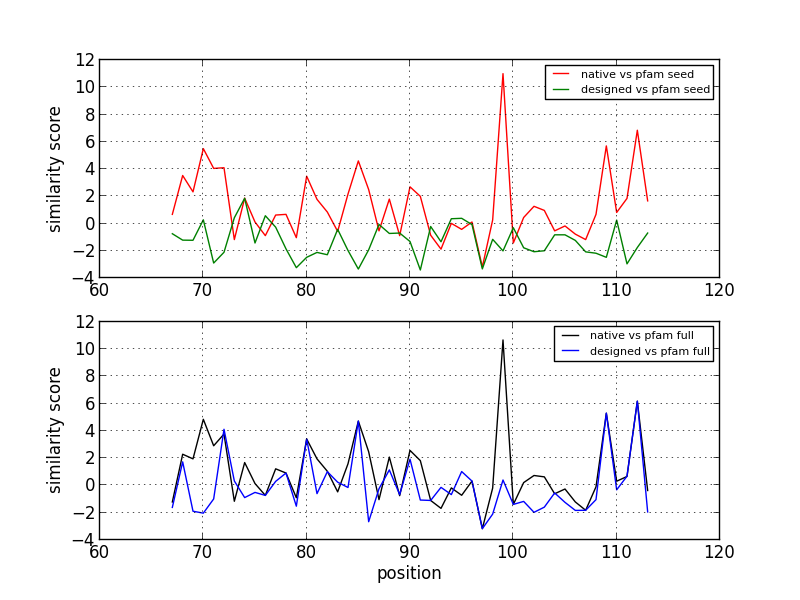
\includegraphics[width=8cm]{simil_bypos_1ABO_h.png}~
          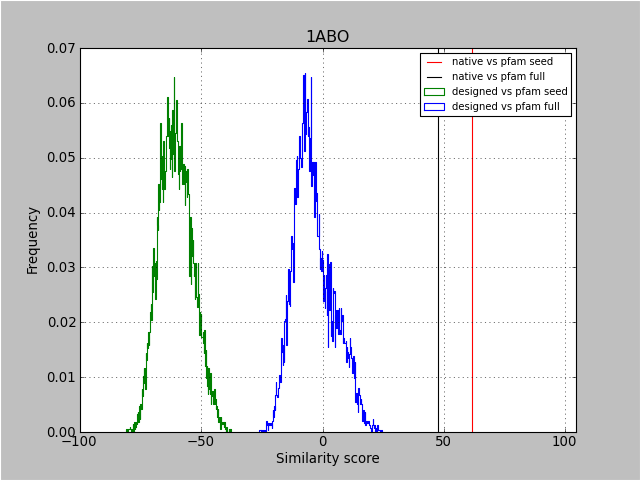
\includegraphics[width=8cm]{simil_byseq_1ABO_h.png} 
     \caption{protocole h}
   \end{subfigure}

   \begin{subfigure}[b]{\linewidth}
     \centering
          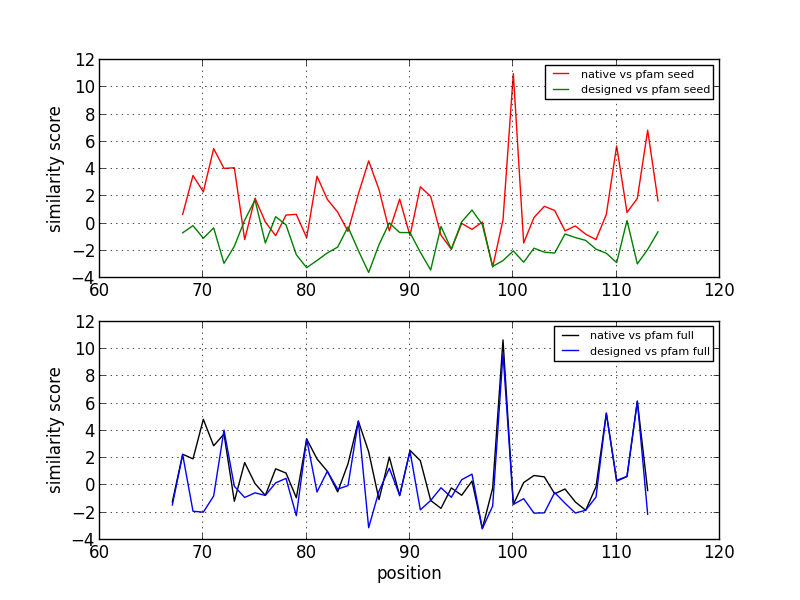
\includegraphics[width=8cm]{simil_bypos_1ABO_mc2.png}~ 
          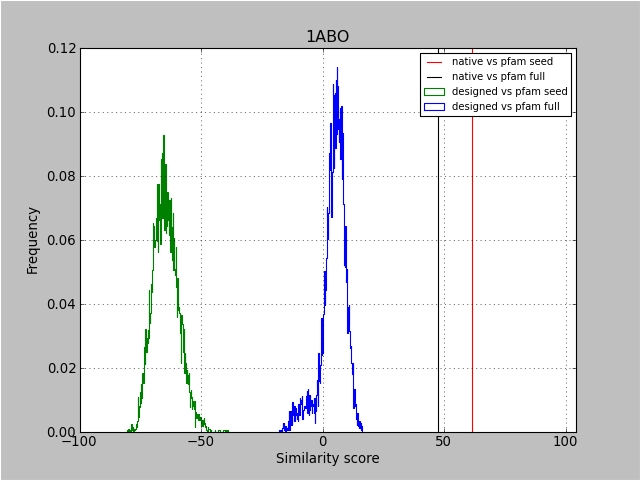
\includegraphics[width=8cm]{simil_byseq_1ABO_mc2.png} 
     \caption{protocole mc2}
   \end{subfigure}

   \begin{subfigure}[b]{\linewidth}
     \centering
          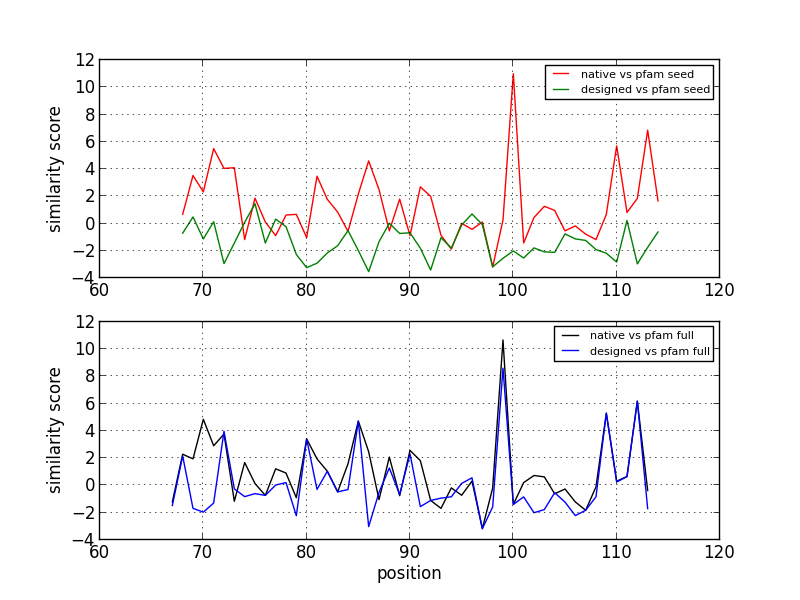
\includegraphics[width=8cm]{simil_bypos_1ABO_mc3.png}~  
          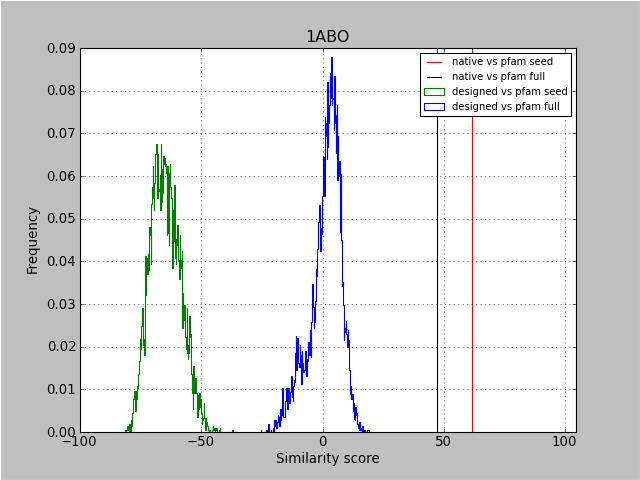
\includegraphics[width=8cm]{simil_byseq_1ABO_mc3.png} 
     \caption{protocole mc3}
   \end{subfigure}

     \caption{Similarité par position et par séquence pour 1ABO}
\label{grah:simil_1ABO}
   \end{figure}

   \begin{figure}
   \begin{subfigure}[b]{\linewidth}
     \centering
          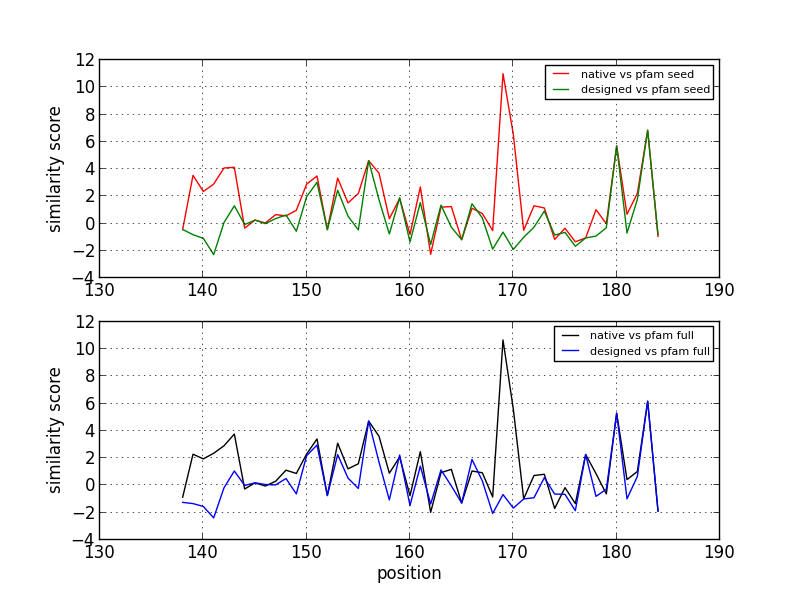
\includegraphics[width=8cm]{simil_bypos_1CKA_h.png}~
          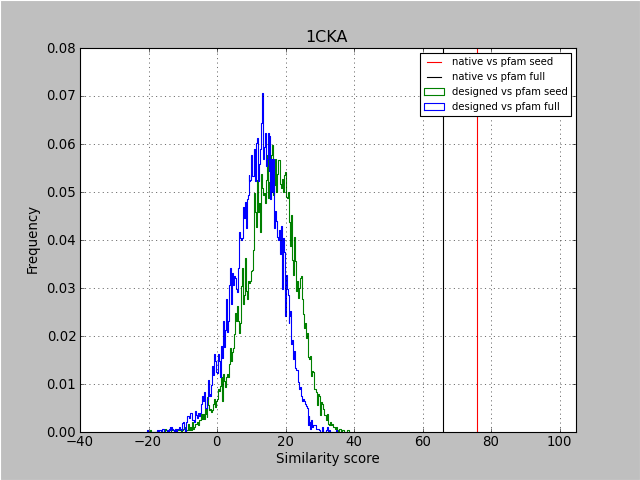
\includegraphics[width=8cm]{simil_byseq_1CKA_h.png} 
     \caption{protocole h}
   \end{subfigure}

   \begin{subfigure}[b]{\linewidth}
     \centering
          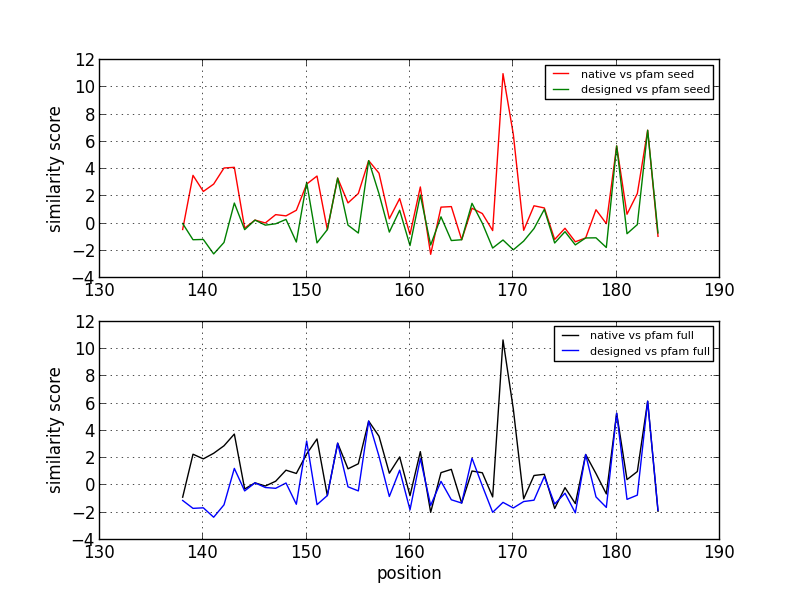
\includegraphics[width=8cm]{simil_bypos_1CKA_mc2.png}~ 
          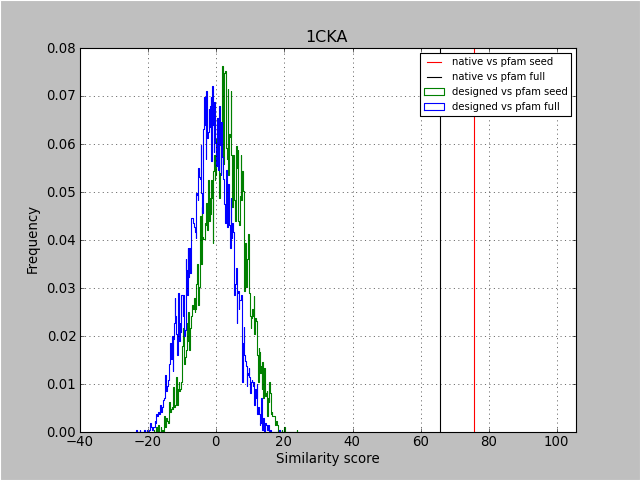
\includegraphics[width=8cm]{simil_byseq_1CKA_mc2.png} 
     \caption{protocole mc2}
   \end{subfigure}

   \begin{subfigure}[b]{\linewidth}
     \centering
          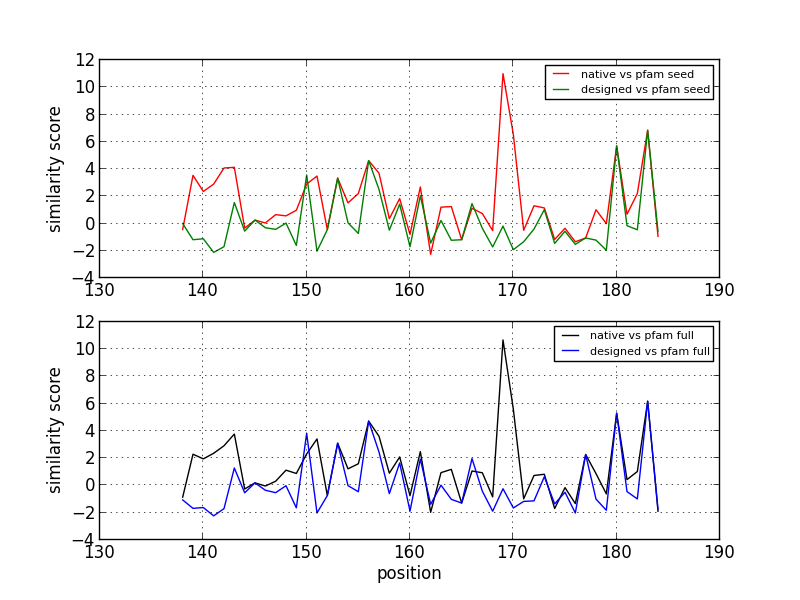
\includegraphics[width=8cm]{simil_bypos_1CKA_mc3.png}~  
          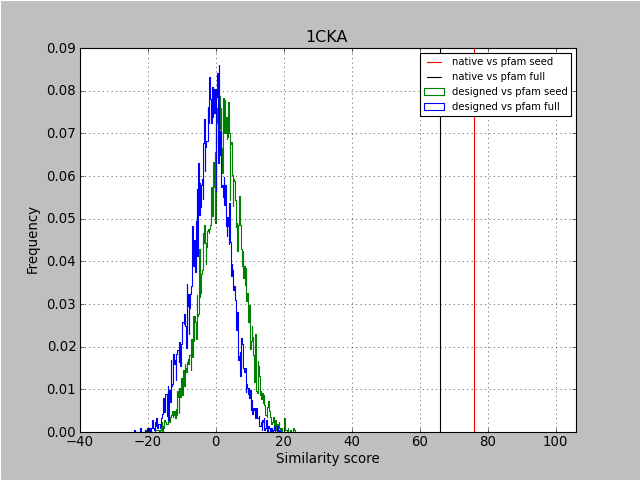
\includegraphics[width=8cm]{simil_byseq_1CKA_mc3.png} 
     \caption{protocole mc3}
   \end{subfigure}

     \caption{Similarité par position et par séquence pour 1CKA}
\label{grah:simil_1CKA}
   \end{figure}

   \begin{figure}
   \begin{subfigure}[b]{\linewidth}
     \centering
          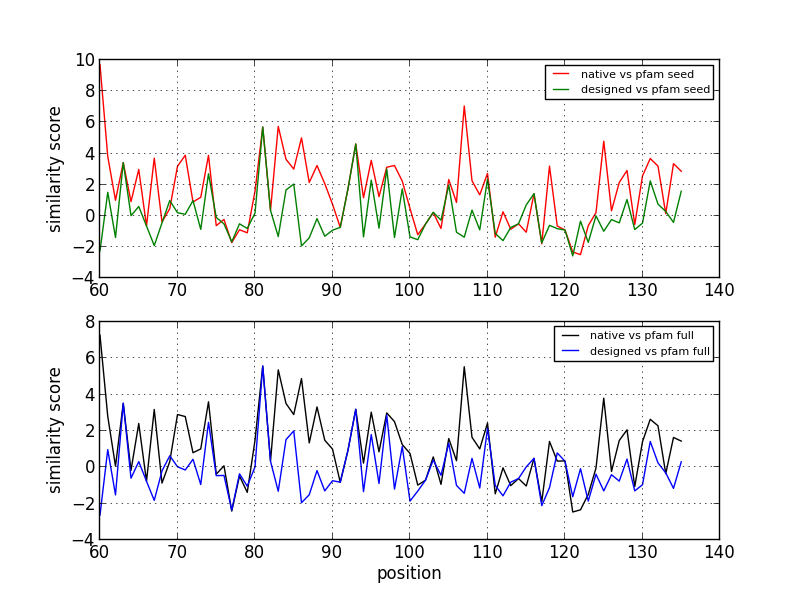
\includegraphics[width=8cm]{simil_bypos_1BM2_h.png}~
          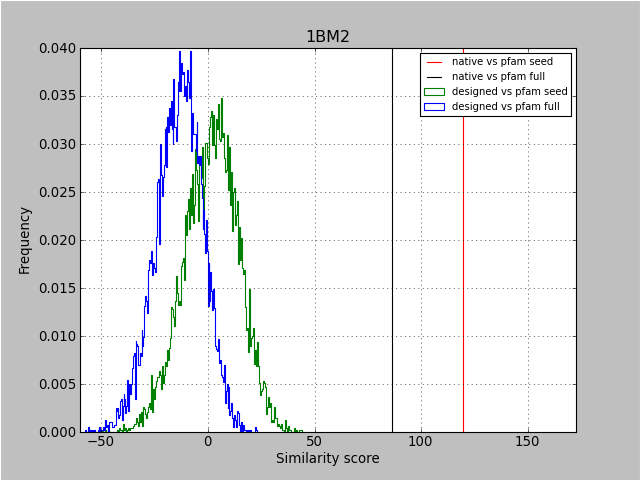
\includegraphics[width=8cm]{simil_byseq_1BM2_h.png} 
     \caption{protocole h}
   \end{subfigure}

   \begin{subfigure}[b]{\linewidth}
     \centering
          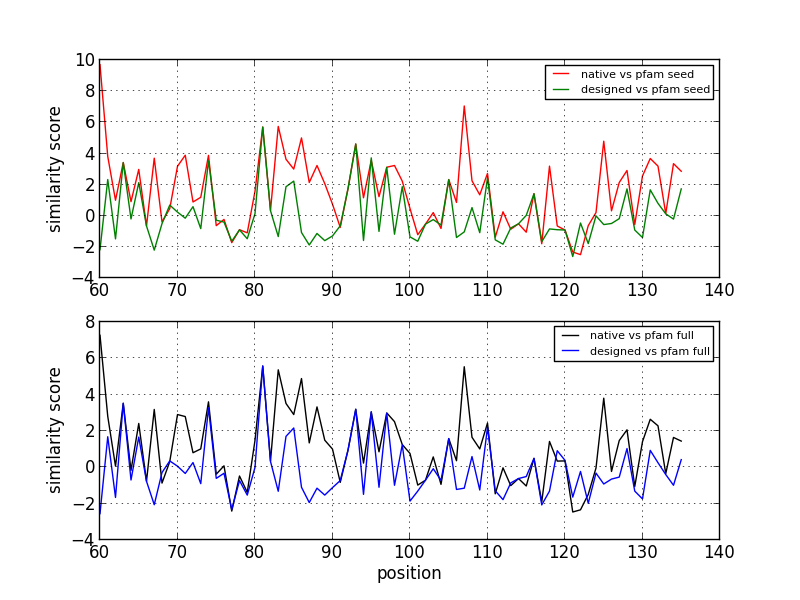
\includegraphics[width=8cm]{simil_bypos_1BM2_mc2.png}~ 
          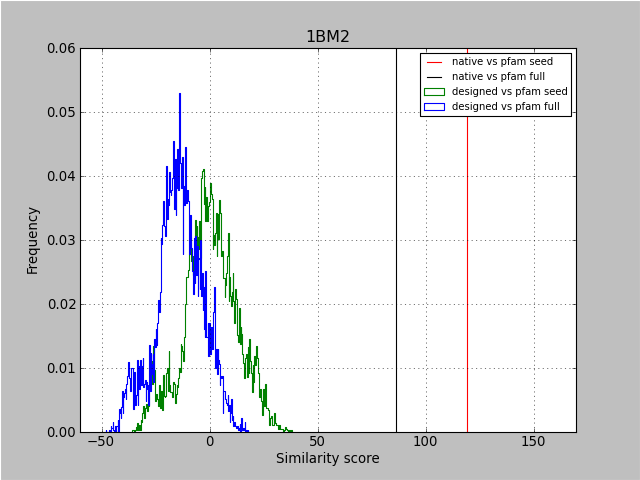
\includegraphics[width=8cm]{simil_byseq_1BM2_mc2.png} 
     \caption{protocole mc2}
   \end{subfigure}

   \begin{subfigure}[b]{\linewidth}
     \centering
          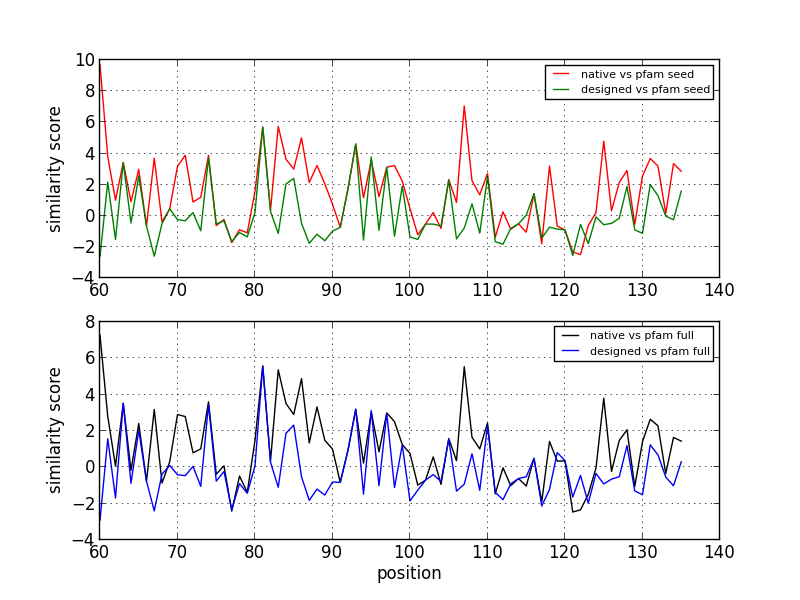
\includegraphics[width=8cm]{simil_bypos_1BM2_mc3.png}~  
          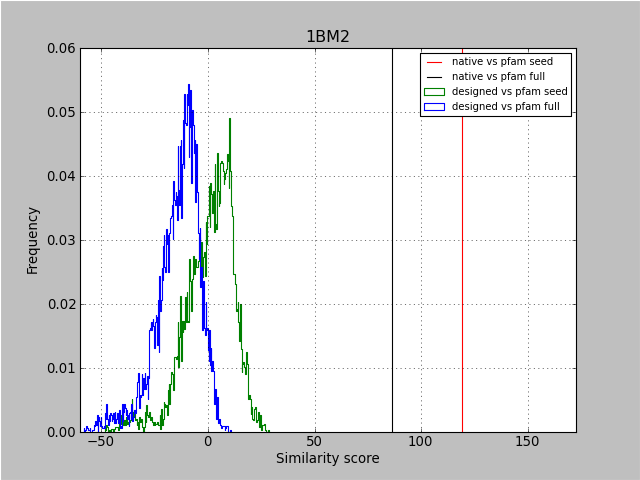
\includegraphics[width=8cm]{simil_byseq_1BM2_mc3.png} 
     \caption{protocole mc3}
   \end{subfigure}

     \caption{Similarité par position et par séquence pour 1BM2}
\label{grah:simil_1BM2}
   \end{figure}

   \begin{figure}
   \begin{subfigure}[b]{\linewidth}
     \centering
          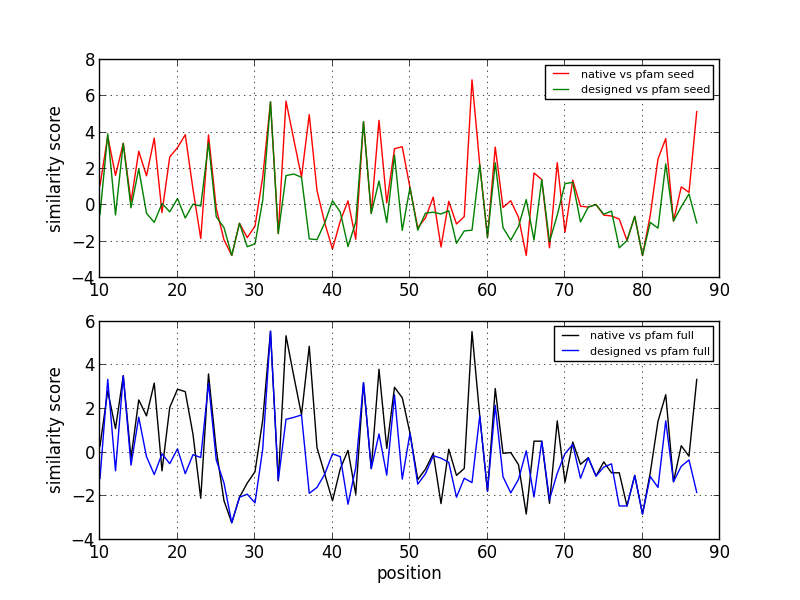
\includegraphics[width=8cm]{simil_bypos_1M61_h.png}~
          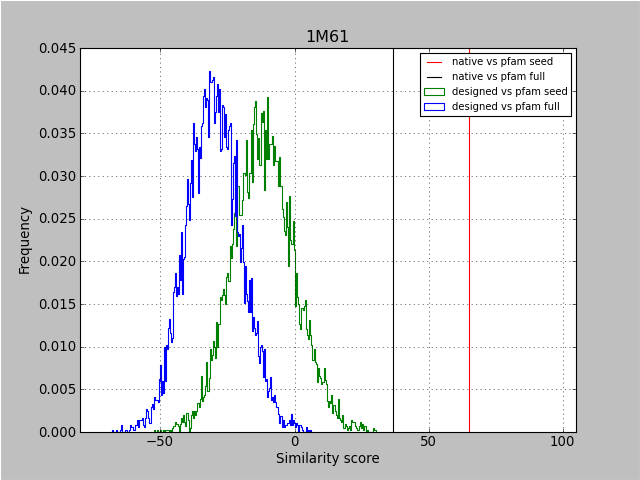
\includegraphics[width=8cm]{simil_byseq_1M61_h.png} 
     \caption{protocole h}
   \end{subfigure}

   \begin{subfigure}[b]{\linewidth}
     \centering
          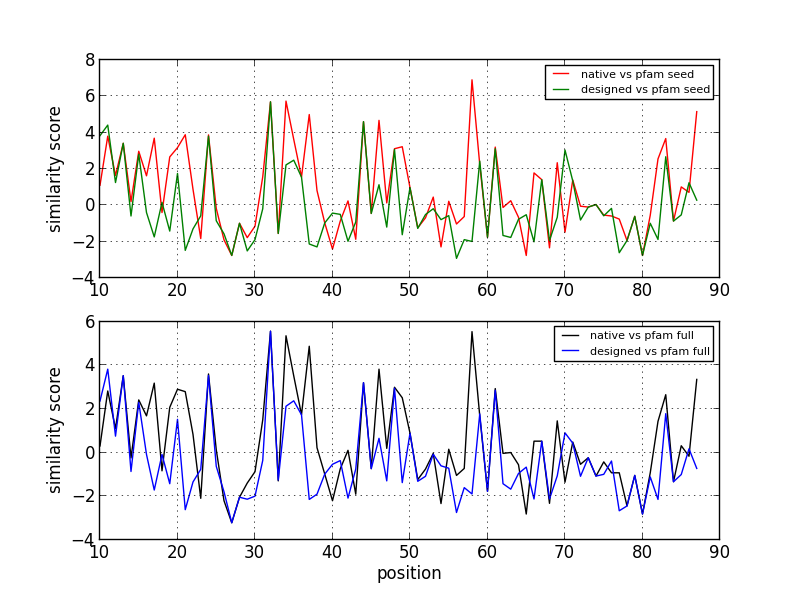
\includegraphics[width=8cm]{simil_bypos_1M61_mc2.png}~ 
          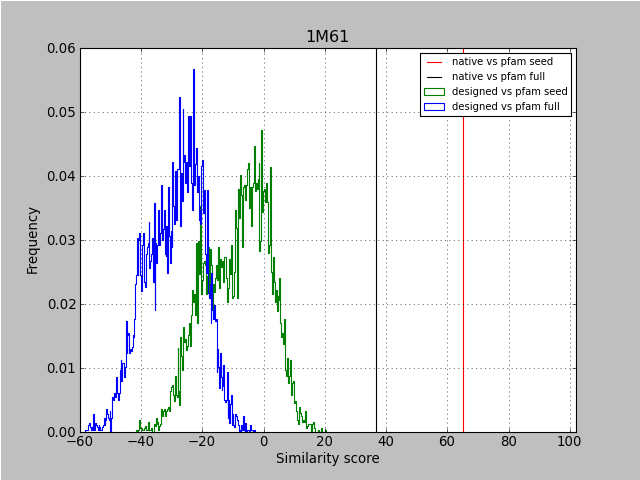
\includegraphics[width=8cm]{simil_byseq_1M61_mc2.png} 
     \caption{protocole mc2}
   \end{subfigure}

   \begin{subfigure}[b]{\linewidth}
     \centering
          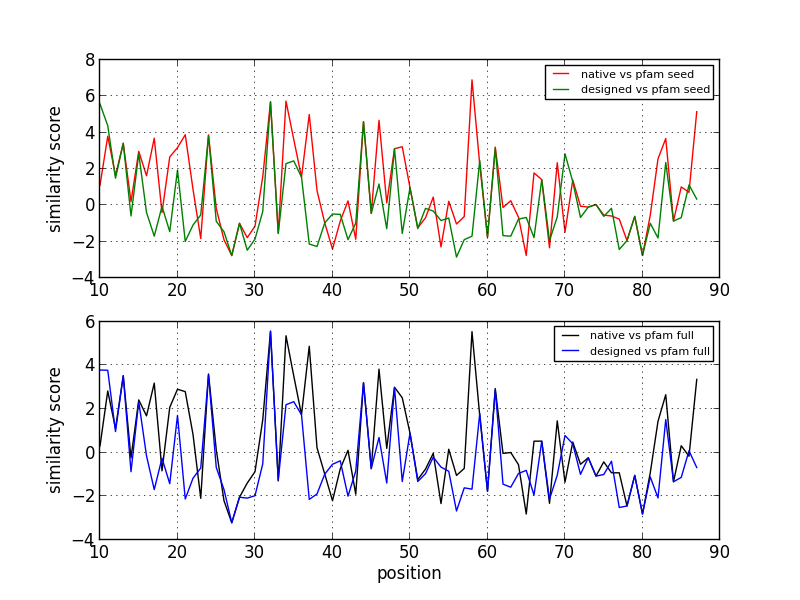
\includegraphics[width=8cm]{simil_bypos_1M61_mc3.png}~  
          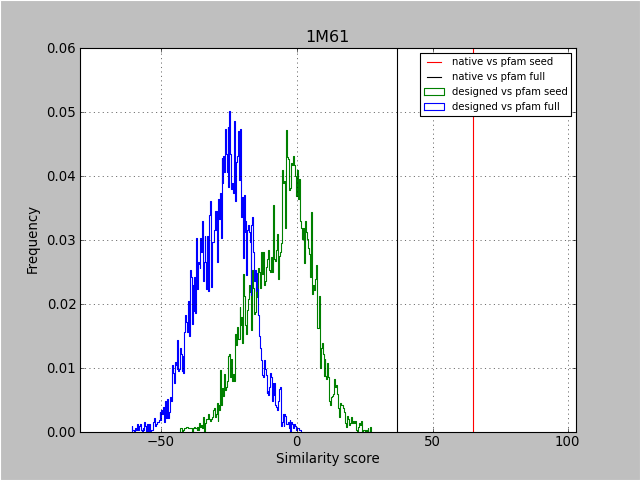
\includegraphics[width=8cm]{simil_byseq_1M61_mc3.png} 
     \caption{protocole mc3}
   \end{subfigure}

     \caption{Similarité par position et par séquence pour 1M61}
\label{grah:simil_1M61}
   \end{figure}

   \begin{figure}
   \begin{subfigure}[b]{\linewidth}
     \centering
          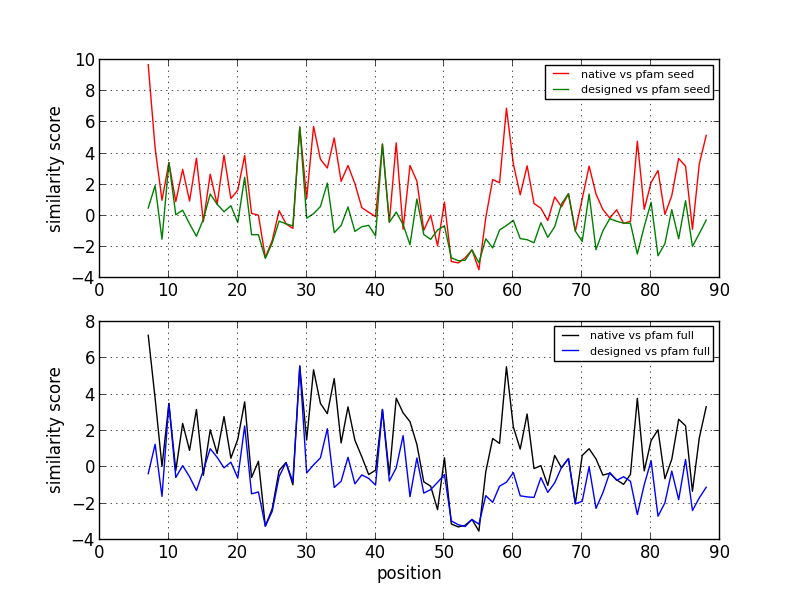
\includegraphics[width=8cm]{simil_bypos_1O4C_h.png}~
          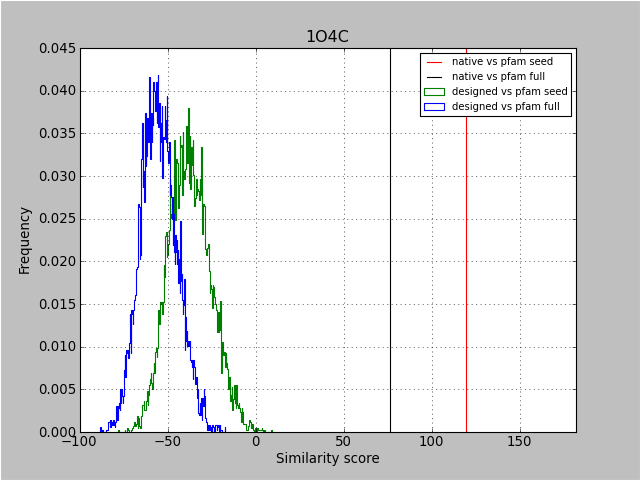
\includegraphics[width=8cm]{simil_byseq_1O4C_h.png} 
     \caption{protocole h}
   \end{subfigure}

   \begin{subfigure}[b]{\linewidth}
     \centering
          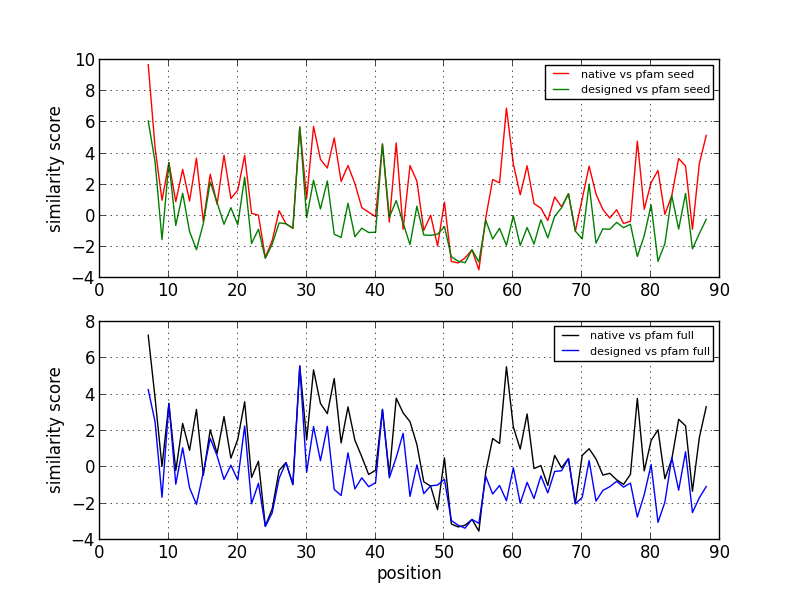
\includegraphics[width=8cm]{simil_bypos_1O4C_mc2.png}~ 
          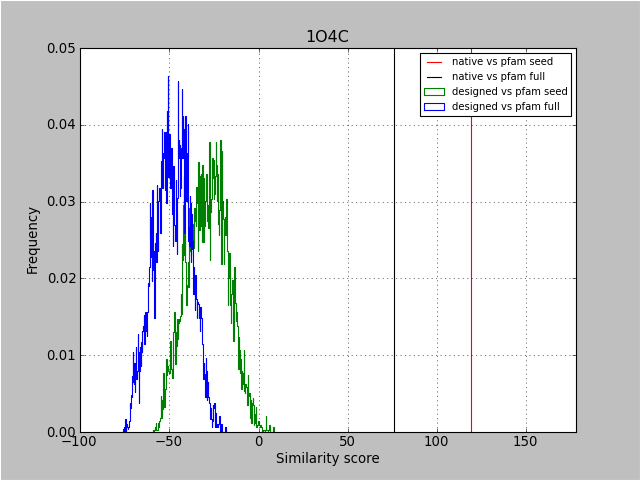
\includegraphics[width=8cm]{simil_byseq_1O4C_mc2.png} 
     \caption{protocole mc2}
   \end{subfigure}

   \begin{subfigure}[b]{\linewidth}
     \centering
          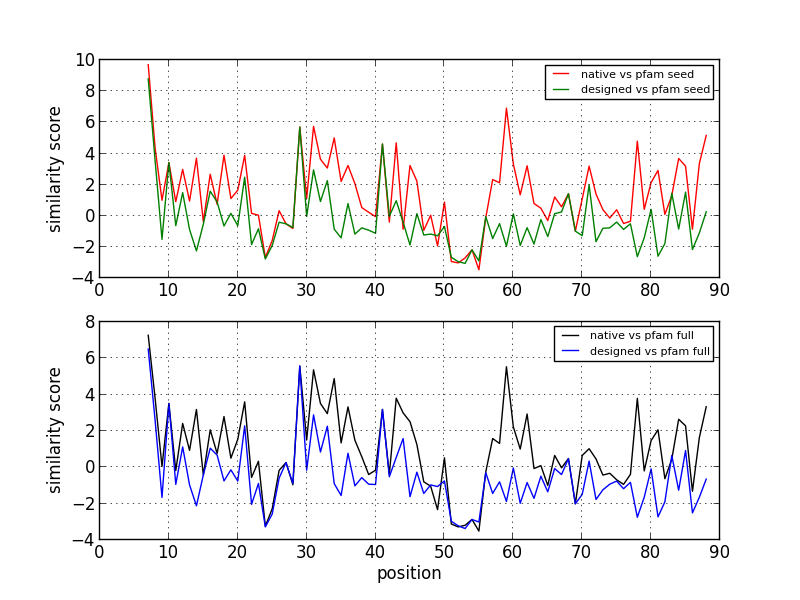
\includegraphics[width=8cm]{simil_bypos_1O4C_mc3.png}~  
          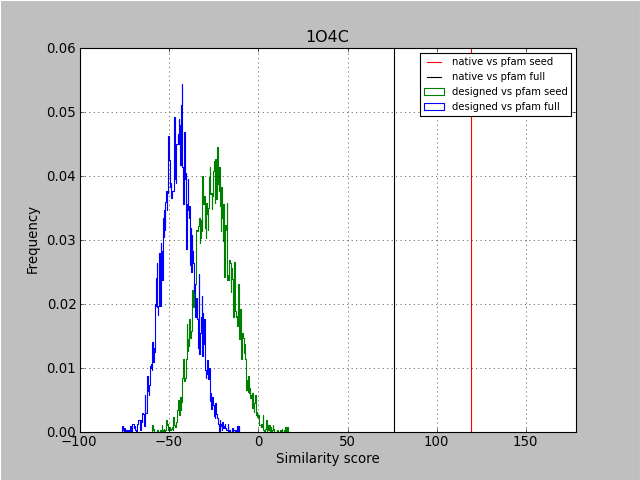
\includegraphics[width=8cm]{simil_byseq_1O4C_mc3.png} 
     \caption{protocole mc3}
   \end{subfigure}

     \caption{Similarité par position et par séquence pour 1O4C}
\label{grah:simil_1O4C}
   \end{figure}

   \begin{figure}
   \begin{subfigure}[b]{\linewidth}
     \centering
          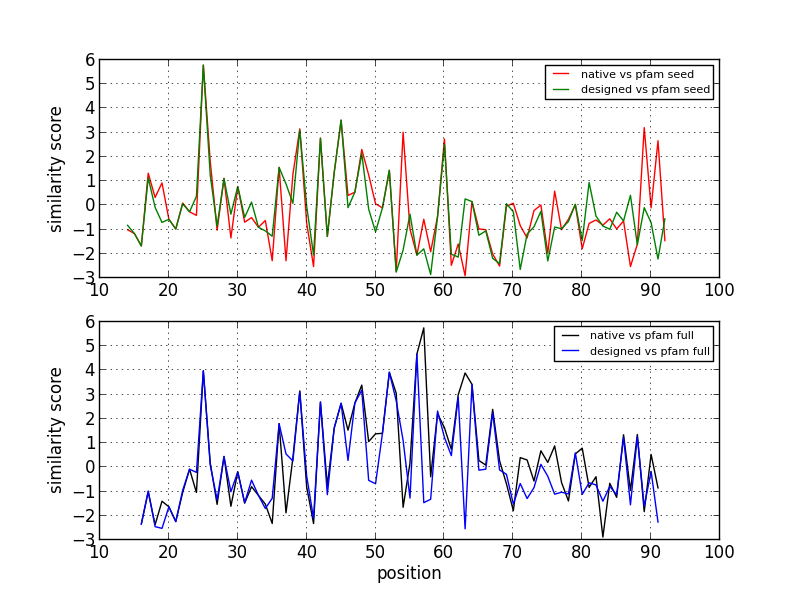
\includegraphics[width=8cm]{simil_bypos_1G9O_h.png}~
          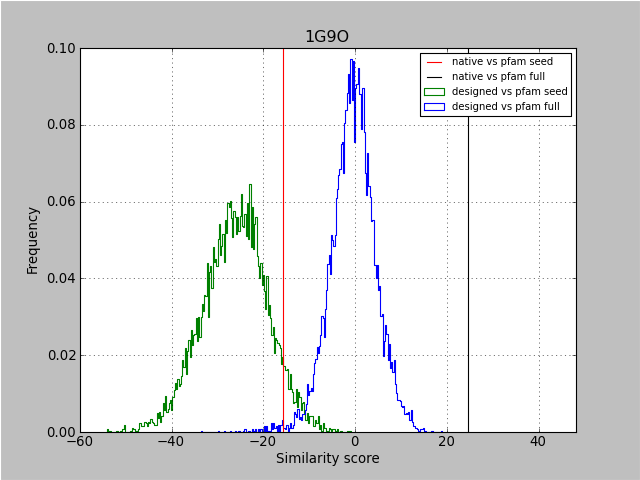
\includegraphics[width=8cm]{simil_byseq_1G9O_h.png} 
     \caption{protocole h}
   \end{subfigure}

   \begin{subfigure}[b]{\linewidth}
     \centering
          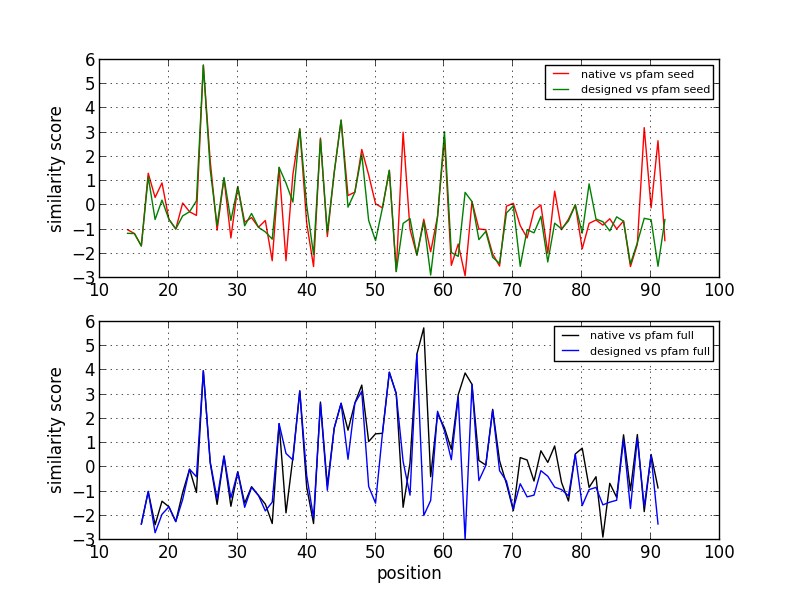
\includegraphics[width=8cm]{simil_bypos_1G9O_mc2.png}~ 
          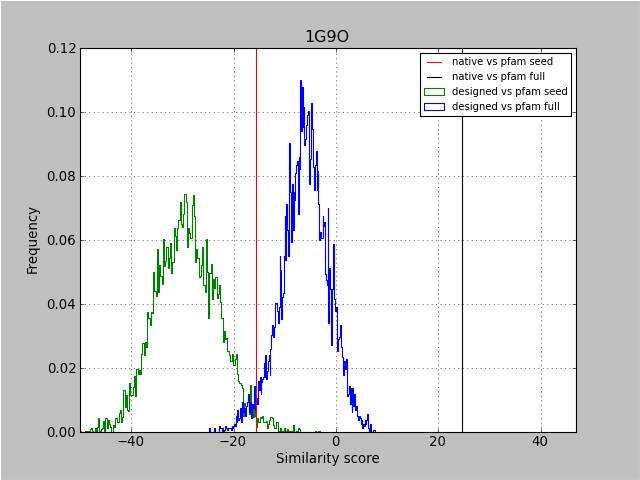
\includegraphics[width=8cm]{simil_byseq_1G9O_mc2.png} 
     \caption{protocole mc2}
   \end{subfigure}

   \begin{subfigure}[b]{\linewidth}
     \centering
          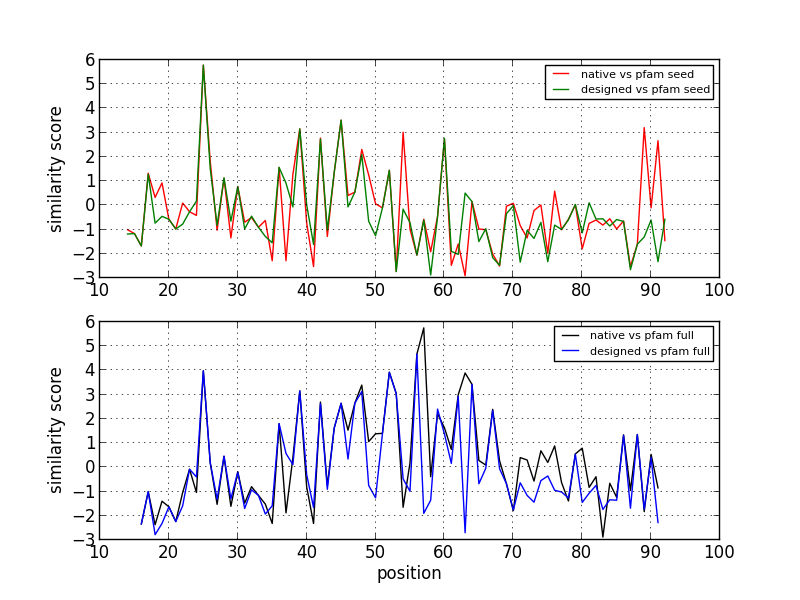
\includegraphics[width=8cm]{simil_bypos_1G9O_mc3.png}~  
          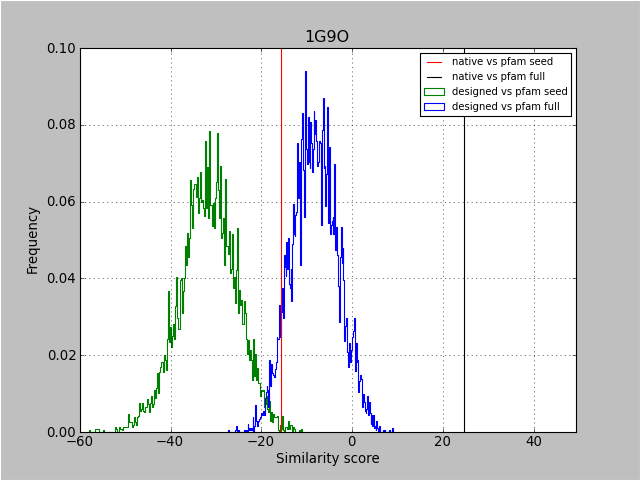
\includegraphics[width=8cm]{simil_byseq_1G9O_mc3.png} 
     \caption{protocole mc3}
   \end{subfigure}

     \caption{Similarité par position et par séquence pour 1G9O}
\label{grah:simil_1G9O}
   \end{figure}

   \begin{figure}
   \begin{subfigure}[b]{\linewidth}
     \centering
          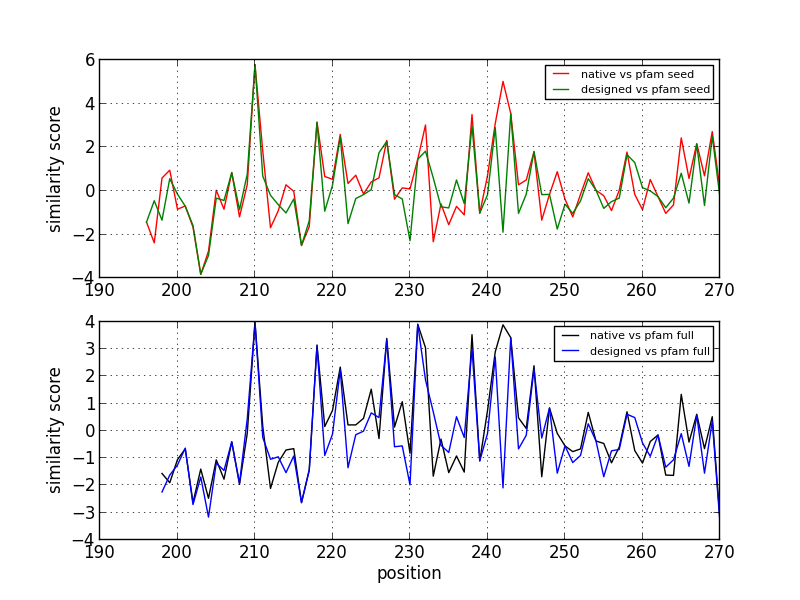
\includegraphics[width=8cm]{simil_bypos_1R6J_h.png}~
          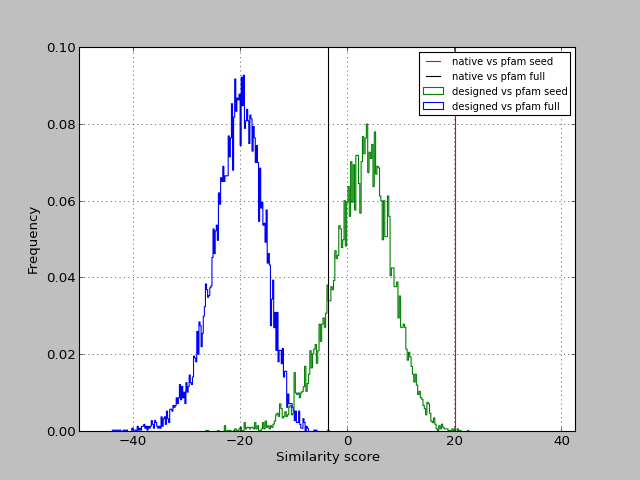
\includegraphics[width=8cm]{simil_byseq_1R6J_h.png} 
     \caption{protocole h}
   \end{subfigure}

   \begin{subfigure}[b]{\linewidth}
     \centering
          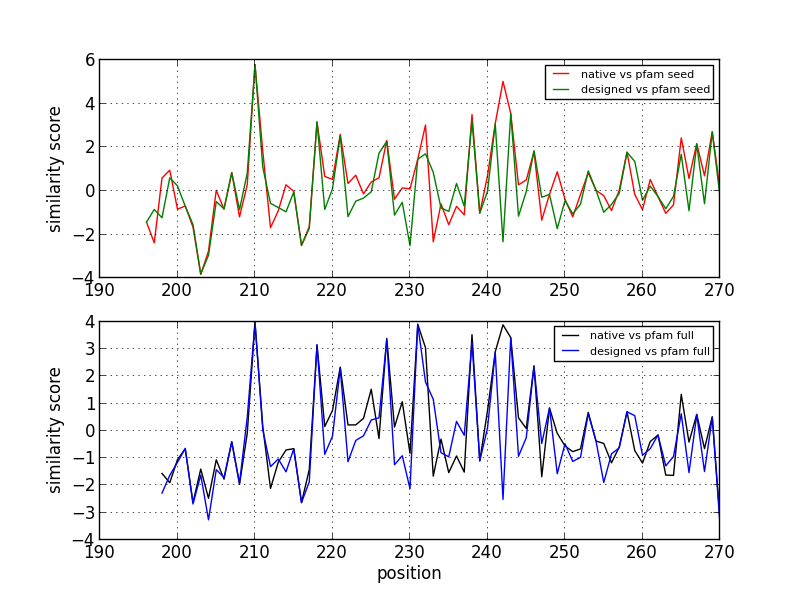
\includegraphics[width=8cm]{simil_bypos_1R6J_mc2.png}~ 
          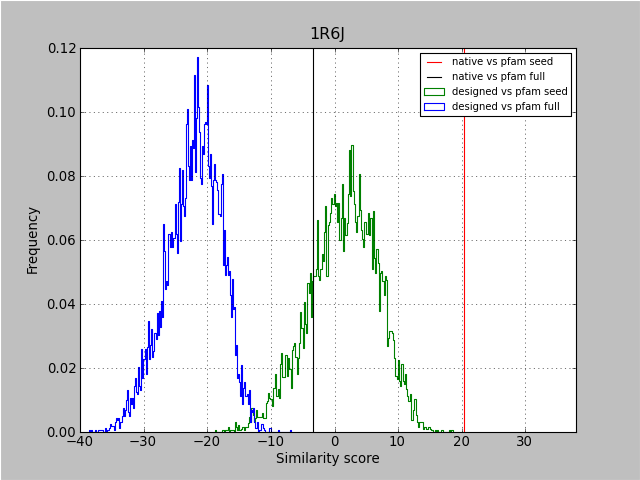
\includegraphics[width=8cm]{simil_byseq_1R6J_mc2.png} 
     \caption{protocole mc2}
   \end{subfigure}

   \begin{subfigure}[b]{\linewidth}
     \centering
          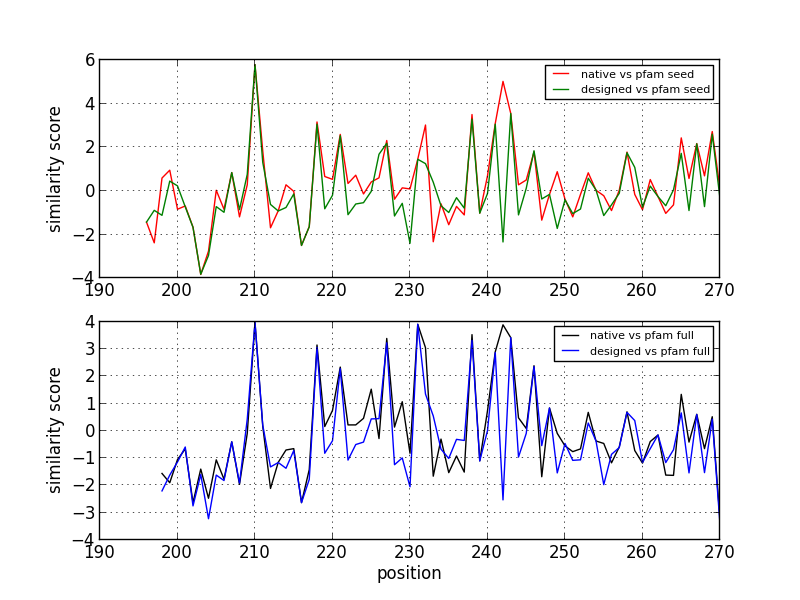
\includegraphics[width=8cm]{simil_bypos_1R6J_mc3.png}~  
          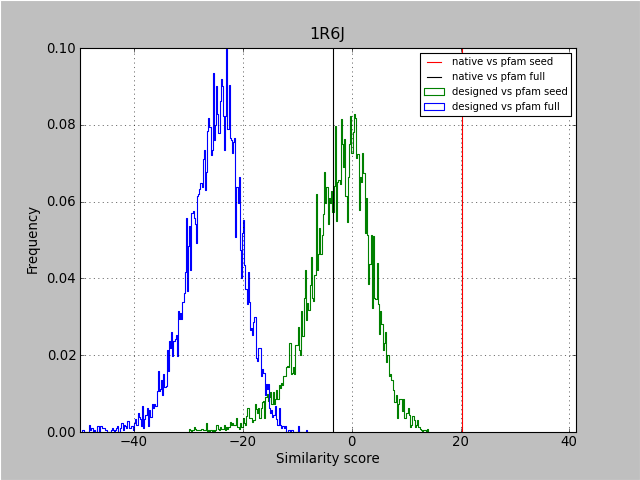
\includegraphics[width=8cm]{simil_byseq_1R6J_mc3.png} 
     \caption{protocole mc3}
   \end{subfigure}

     \caption{Similarité par position et par séquence pour 1R6J}
\label{grah:simil_1R6J}
   \end{figure}

\paragraph{rapport entre énergies et  similarités}
Pour faire le lien entre les comparaisons basées sur les meilleures énergies et les comparaisons basées sur les scores de similarités, nous représentons les énergies des dix mille meilleures séquences en fonction de leur similarité à l'alignement Pfam « seed». Une séquence peut apparaître plusieurs fois dans l'ensemble des séquences/conformations obtenues.Alors toutes les énergies trouvées de la séquence sont représentées voir les graphiques \ref{graph:simil_vs_ener}. La corrélation entre les deux critères semble très faible.Pour 1CKA malgré des énergies pour l'heuristique moins bonnes, la similarité est meilleure.Bien que les énergies obtenues avec le protocole mc2 soient meilleures que celles avec le protocole mc3, il n'y a pas de différence significative sur les scores de similarités obtenus.

   \begin{figure}[t]
     \centering
     \begin{tabular}{cc}
       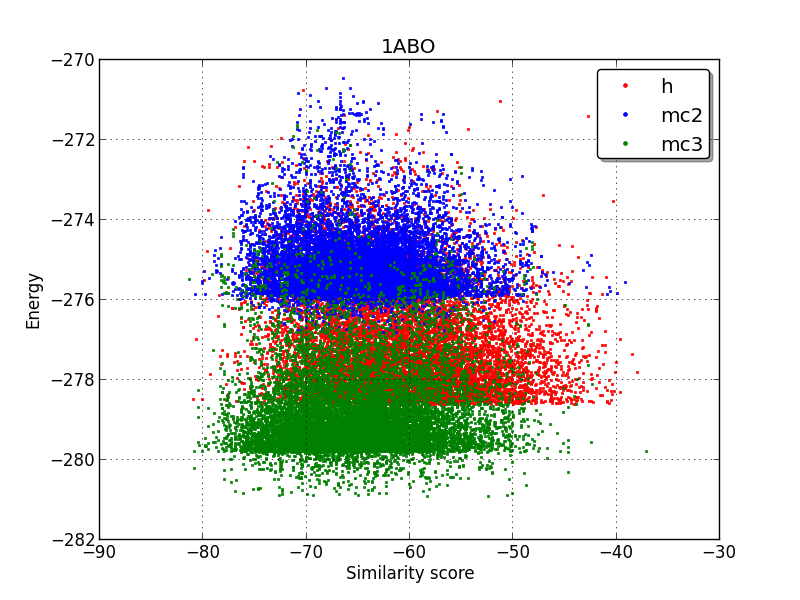
\includegraphics[width=7cm]{simil_vs_ener_1ABO.png} &
       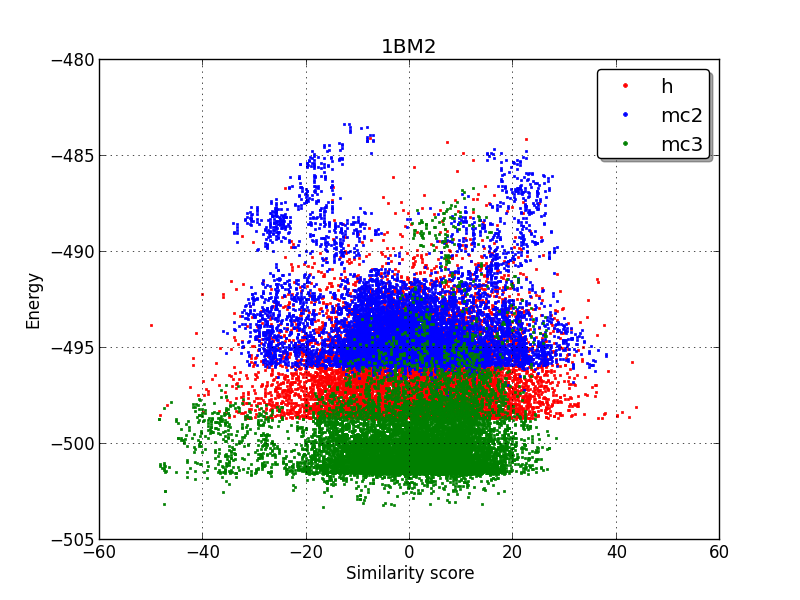
\includegraphics[width=7cm]{simil_vs_ener_1BM2.png} \\
       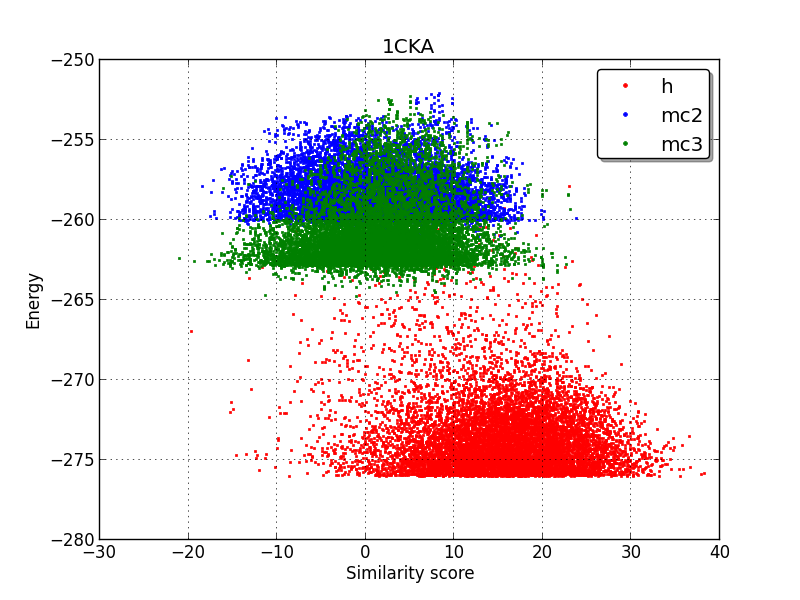
\includegraphics[width=7cm]{simil_vs_ener_1CKA.png} &
       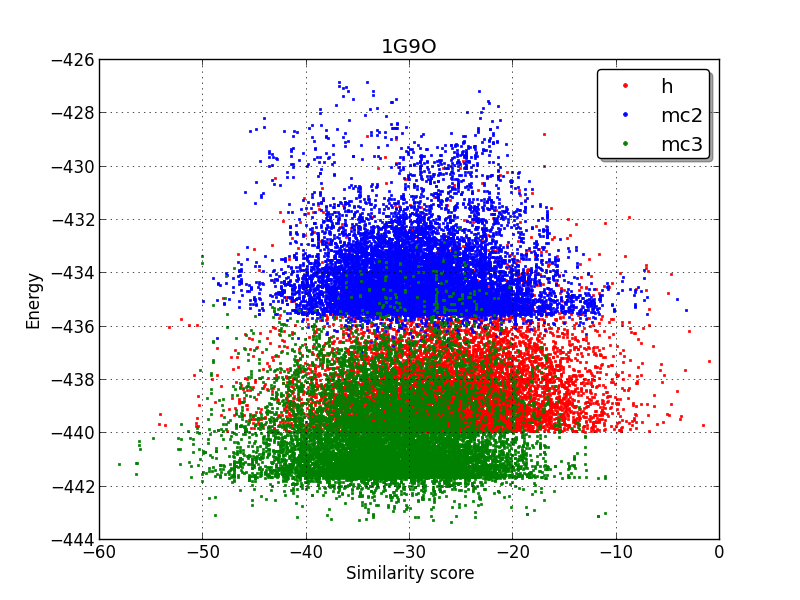
\includegraphics[width=7cm]{simil_vs_ener_1G9O.png} \\
       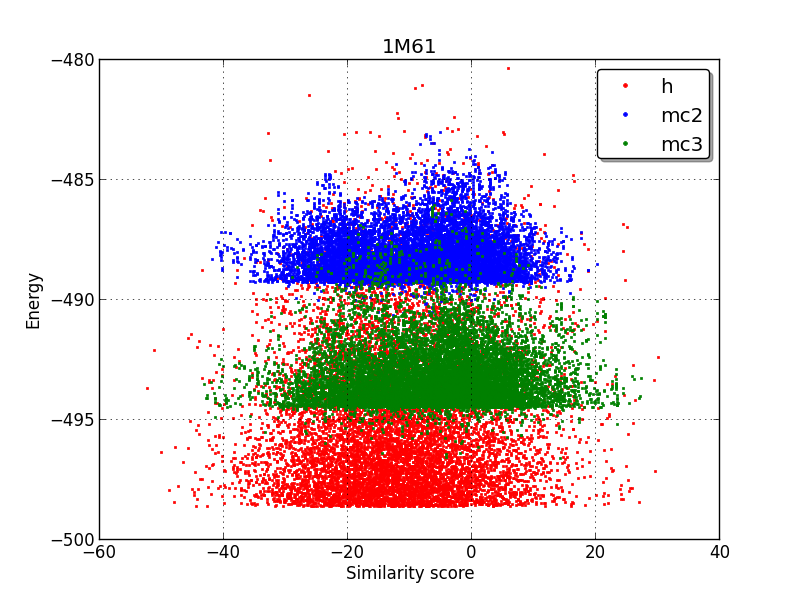
\includegraphics[width=7cm]{simil_vs_ener_1M61.png} &
       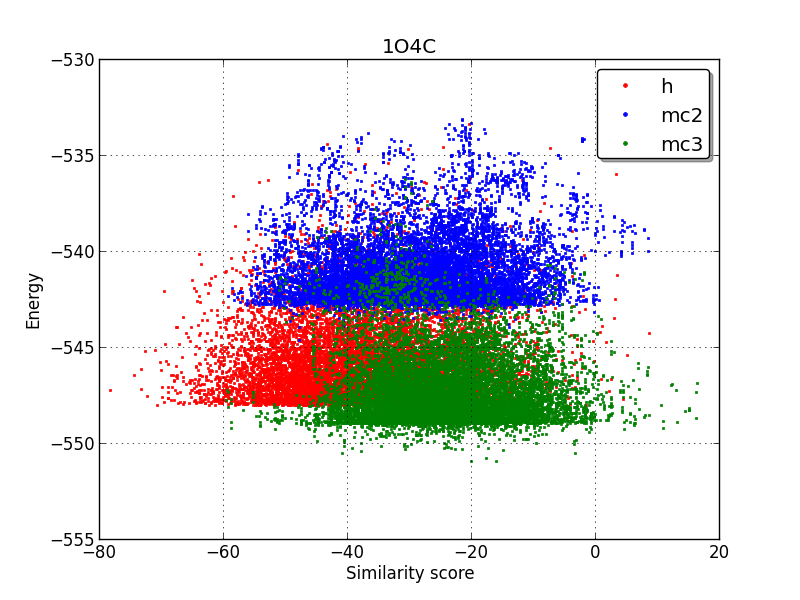
\includegraphics[width=7cm]{simil_vs_ener_1O4C.png} \\
       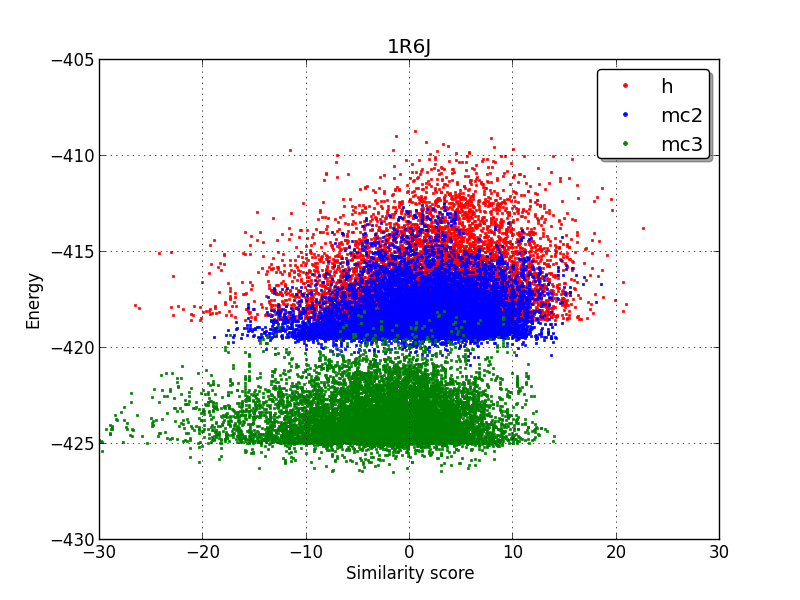
\includegraphics[width=8cm]{simil_vs_ener_1R6J.png} \\
     \end{tabular}
     \caption{Similarité selon l'énergie}
\label{graph:simil_vs_ener}
   \end{figure}
 

\paragraph{Comparaisons des distributions selon l'énergie}

Ici nous nous intéressons aux ensembles de cent mille séquences/conformations de meilleures énergies.Nous calculons les centiles d'énergie pour chaque protéine et pour chacun des trois protocoles h , mc2, mc3.  

Les figures~\ref{graph:centiles} représentent la répartition des énergies selon les centiles, ceci pour les trois protocoles h, mc2, mc3. Pour le premier centile  ( c'est-à-dire l'énergie au-dessus de laquelle il y a les mille meilleures séquences/conformations) le protocole mc2 domine sauf pour la protéine 1R6J où h est meilleur jusqu'au vingtième centile .Pour 1ABO, alors que mc2 et mc3 font quasiment jeu égal pour la meilleure énergie, le premier centile de mc2 est nettement plus haut que celui de mc3.Mais en général, l'allure des courbes des deux protocoles Monte-Carlo est très proche.Et les écarts entre  les meilleures énergies de mc2 et mc3 sont globalement conservés le long des centiles.Ce n'est pas le cas entre h et les protocoles Monte-Carlo, où l'on voit un déclin plus rapide le long des centiles.Ce qui montre une densité plus faible des séquences/conformations de bonne énergie pour l'heuristique. 


   \begin{figure}[t]
     \centering
     \begin{tabular}{cc}
       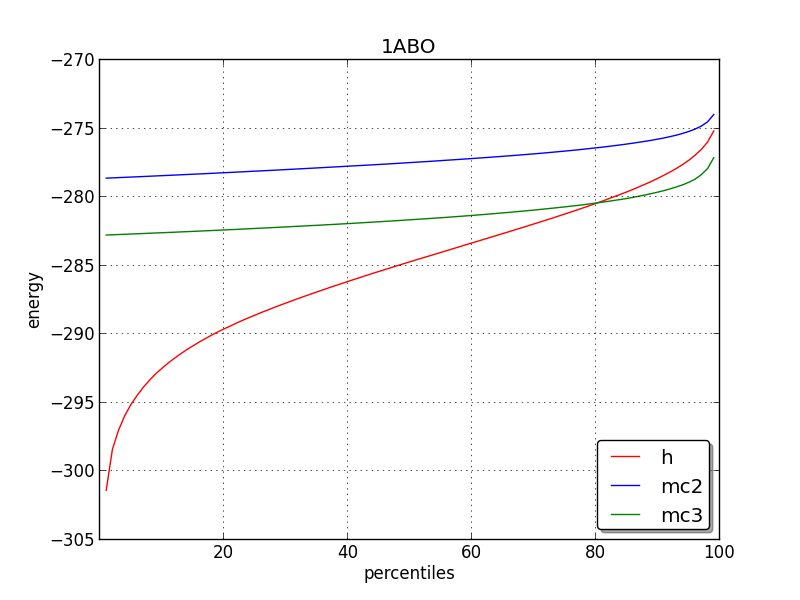
\includegraphics[width=8cm]{centiles_1ABO.png} &
       \includegraphics[width=8cm]{centiles_1BM2.png} \\
       \includegraphics[width=8cm]{centiles_1CKA.png} &
       \includegraphics[width=8cm]{centiles_1G9O.png} \\
       \includegraphics[width=8cm]{centiles_1M61.png} &
       \includegraphics[width=8cm]{centiles_1O4C.png} \\
       \includegraphics[width=8cm]{centiles_1R6J.png} \\
     \end{tabular}
     
     \caption{Distribution des 100000 meilleures séquences selon l'énergie.}
\label{grah:centiles}
   \end{figure}
 
\clearpage

\subsection{Comparaisons avec toutes les positions actives}


\paragraph{meilleure énergie selon les protocoles}
Passons maintenant, aux résultats obtenus avec la seconde version de proteus~\ref{qqchose}.Cette version intègre notamment l'algorithme « Replica Exchange». Nous pouvons donc faire des comparaisons entre les trois algorithmes du programme.Tous les protocoles utilisés sont décrits dans les tableaux~\ref{tab:protoMC} ou \ref{tab:protoRE}.Commençons par la recherche de la séquence/conformation de meilleure énergie pour toutes les positions actives. Les tests sont décrits au paragraphe~\ref{methode_TTactif}. Les résultats sont présentés sous forme de tableau en~\ref{tab:best_ener_all_all} qui contient la meilleure énergie arrondie à la kcal/mol inférieure et aussi sous forme de graphique en~\ref{graph:best_ener_all_all} où sont représenter les différences par rapport à la meilleure énergie pour tous les cas. 

Il n'y pas de protocole qui domine les autres sur toutes les protéines. Le meilleur résultat est obtenu avec le protocole huit marcheurs RE8b2 pour 2BYG , 1BM2, 1O4C et 1A81, le protocole RE8b1 pour 1CKA et 1ABO, le protocole quatre marcheurs RE4b pour 1G9O , les protocoles mono marcheurs MCb pour 1M61 et H pour 1R6J.  Ces résultats sont également représentés sous forme de trois graphiques qui regroupent les protocoles utilisant les protocoles non parallèles, les protocoles quatre marcheurs et les protocoles huit marcheurs. Un quatrième graphique regroupe le meilleur protocole de chaque algorithme. Là encore, seules les différences par rapport au meilleur protocole sont représentées. Le protocole H fait jeu égal avec le meilleur protocole Monte-Carlo. Le second Monte-Carlo , qui utilise en mode de mutation moins agressif~\ref{para:MC}, est nettement plus mauvais avec presque toujours des écarts de plus de cinq Kcal/mol avec les deux autres protocoles non parallèles.Pour le groupe de protocoles avec quatre marcheurs, le RE4b qui se différencie des deux autres par une plage de températures la plus resserrée est meilleur pour cinq des sept protéines. Mais pour les deux protéines restantes la différence se limite à deux Kcal/mol.RE4a, le protocole avec la plage de température la large est moins bon que les autres. En ce qui conserve les protocoles huit marcheurs , deux d'entre eux se démarquent RE8b1 et RE8b2 (plage de température resserrée,grande période de swap et mode de modification agressif pour le premier , plus conservateur pour le second). RE8b1 obtient des résultats assez irréguliers selon les protéines du meilleur pour 1CKA et 1ABO jusqu'à s'écarter de près de huit Kcal/mol de la plus haute énergie.RE8b2, soit donne les meilleurs résultats (dans cinquante pour cent des cas), soit s'écarte d'au plus quatre Kcal/mol des meilleurs résultats.  

    \begin{table}[h]
      \centering

      \begin{tabular}{cccccccccccc}


        \toprule
        Protéine & H & MCa & MCb & RE4a & RE4b & RE4c & RE8a1 & RE8a2 & RE8b1 & RE8b2 & RE8b3 \\
        \cmidrule{1-12}
        1A81 & -521 & -538 & -522 & -525 & -520 & -518 & -520 & -520 & -514 & -512 & -512 \\
        1ABO & -272 & -274 & -268 & -273 & -269 & -272 & -273 & -273 & -268 & -271 & -271 \\
        1BM2 & -484 & -500 & -486 & -488 & -481 & -486 & -489 & -489 & -478 & -476 & -480 \\
        1CKA & -252 & -258 & -249 & -259 & -251 & -249 & -251 & -251 & -247 & -248 & -252 \\
        1G9O & -428 & -435 & -428 & -429 & -421 & -428 & -430 & -430 & -428 & -425 & -426 \\
        1M61 & -480 & -493 & -479 & -483 & -480 & -480 & -481 & -481 & -480 & -480 & -480 \\
        1O4C & -535 & -545 & -531 & -536 & -529 & -532 & -536 & -536 & -527 & -524 & -525 \\
        1R6J & -407 & -419 & -414 & -415 & -409 & -414 & -411 & -411 & -409 & -408 & -409 \\
        2BYG & -457 & -469 & -454 & -461 & -456 & -462 & -460 & -460 & -456 & -454 & -454 \\
        
        \bottomrule
      \end{tabular}      
      \caption{les meilleures énergies pour tous les résidus actifs}
\label{tab:best_ener_all_all}      
    \end{table}


   \begin{figure}[t]
     \centering
     \begin{tabular}{cc}
       \includegraphics[width=18cm]{best_all.png} \\
     \end{tabular}
     \caption{Les différences entre les meilleures énergies de chaque protocole.}
\label{graph:best_ener_all_all}
   \end{figure}


    \clearpage


   \begin{figure}[t]
     \centering
     \begin{tabular}{cc}
       \includegraphics[width=8cm]{best_by_cat.png} &
       \includegraphics[width=8cm]{monoM.png} \\
       \includegraphics[width=8cm]{best_RE4.png} &
       \includegraphics[width=8cm]{best_RE8.png} \\
     \end{tabular}
     \caption{.Les différences entre les meilleures énergies par groupe de protocoles}
\label{graph:best_ener_by_algo}
   \end{figure}


\paragraph{Distribution des énergies en fonction des températures}

Regardons plus en détail le comportement du programme pour l'algorithme "Replica Exchange". Notre implémentation de cet algorithme consiste à modifier la température de certains marcheurs à certains moments voir~\ref{???}.Pour examiner la trajectoire à une température donnée t ( c'est à dire le graphe dans l'espace les séquences/conformations selon les pas du marcheur lorsqu'ils sont à la température t), nous découpons les trajectoires des marcheurs  selon la température. Puis nous collons les segments de trajectoires de même température en respectant l'ordre des pas.Comme les changements de températures se font de façon synchrone , c’est-à-dire un échange entre deux marcheurs, nous obtenons autant de trajectoires selon la température qu'il y a de marcheurs et ces nouvelles trajectoires sont de mêmes longueurs que les trajectoires obtenues par proteus. La figure~\ref{graph:Distrib_E_T} représente la distribution en énergie des trajectoires selon la température sur le test utilisant le protocole RE8b1 sur la protéine 1A81. Nous observons une courbe en cloche pour chaque température, retrouvant ainsi l'allure d'une distribution de Boltzman.  L'espace de recouvrement entre deux courbes consécutives, représente la partie de la distribution dans laquelle les échanges de température vont être se concentrer, parce que cette zone recouvre les situations où la température peut augmente sans dégradation de l'énergie. En effet, le critère de Metropolis-Hasting peut accepter un réchauffement de marcheur (respectivement un refroidissement) si son énergie diminue  (respectivement, augmente) , mais uniquement avec une probabilité qui décroît exponentiellement en fonction de la différence d'énergie.À l'inverse si les recouvrements des distributions consécutives sont trop importants le marcheur peut difficilement s'éloigner de la plage d'énergie d'une température.Le graphique nous confirme que le choix d'une plage de température entre 3.0 et 0.175 pour les protocoles huit marcheurs rend possibles les échanges de températures et permet également l'exploration d'une vaste zone d'énergie.   




   \begin{figure}[t]
     \centering
     \begin{tabular}{cc}
       \includegraphics[width=12cm]{1A81_RE8b1.png} &
     \end{tabular}
     
     \caption{Distribution des énergies selon la température (1A81 protocole RE8b1).}
\label{graph:Distrib_E_T}
   \end{figure}

\paragraph{Trajectoires dans l'espace des températures}

Un critère de performance souvent utilisé est la proportion de changements de températures effectivement acceptés. Pour examiner ces changements, nous représentons la trajectoire dans l'espace des températures pour quatre tests sur la protéine 1A81. Il s'agit des tests effectués avec deux protocoles à quatre marcheurs, le RE4a et le RE4b et deux protocoles à huit marcheurs, le RE8a2 et le REb1, voir figure~\ref{graph:TRAJ_T}.Les deux graphiques quatre marcheurs représentent seulement la moitié des trajectoires de 1,5 million de pas , tandis que les graphiques huit marcheurs représentent la totalité de trajectoires de 750 millions de pas.Comme prévu, le protocole RE4a , qui possède des températures plus écartées , brasse assez mal les températures. En particulier, le marcheur w4 ne quitte presque pas la température la plus froide, et ce malgré une période de swap assez faible et un nombre d'échanges effectifs assez important. On voit que pour RE4b, protocole avec les températures plus proches , la répartition des échanges est nettement plus uniforme. Le fait de double le nombre de températures pour le même intervalle que RE4a ne suffit pas à résoudre le problème et les trois marcheurs les plus froids en début de trajectoire pour le RE8a2 restent froids. Les bons résultats obtenus pour RE4b sont confirmés pour RE8b1 qui utilise également des températures proches.     


   \begin{figure}[t]
     \centering
     \begin{tabular}{cc}
       \includegraphics[width=8.45cm]{1A81-RE4a-T_traj.png} &
       \includegraphics[width=8.45cm]{1A81-RE4b-T_traj.png} \\
       \includegraphics[width=8.45cm]{1A81-RE8a2-T_traj.png} &
       \includegraphics[width=8.45cm]{1A81-RE8b1-T_traj.png} \\
     \end{tabular}
     \caption{Variation de la température pendant la trajectoire de chaque marcheur (cas exemple de protocoles).}
\label{graph:TRAJ_T}
   \end{figure}


    \clearpage
   \paragraph{Résultats Superfamily}
Le protocole RE8b2 obtient globalement les meilleurs résultats en terme d'énergie. Alors, regardons la similarité des séquences obtenues grâce à lui avec la structure 3D du domaine de chacun des neuf domaines.Les dix mille séquences/conformations de meilleures énergies sont sélectionnées, puis les séquences d'acides aminés uniques dans ces ensembles sont extraites.Nous obtenons des ensembles d'en moyenne six cent quarante-trois séquences d'acides aminés. Superfamily est lancé sur ces séquences.Les résultats sont dans le tableau~\ref{tab:superfamily_bestRE};les colonnes «Superfamily Evalue » et «Family Evalue» contiennent la moyenne des evalues sur l'ensemble.Ils sont très bons avec cent pour cent des séquences attribuées à la structure 3D de la superfamille et de la famille de la séquence native, pour huit des neuf domaines. Seules les séquences de 1A81  ne sont similaires aux familles SCOP.On peut également noter que  bien qu'il existe des écarts de trois et quatre kcal/mol entre les meilleures séquences de RE8b2 et d'autres protocoles pour 1ABO et 1G9O, cela n'affecte en rien la similarité en sens de Superfamily.

    \begin{table}[h]
           \raggedleft{}

      \begin{tabular}{ccccccc}

        \toprule
        Protein & seq  & Match/seq & Superfamily & superfamily & Family & family \\
        Protein & number & size & Evalue & success & Evalue &  success\\
        \cmidrule{1-7}
        1A81 & 708 & no & & & & \\
        1ABO & 406 & 51/58  & 4.4e-4 & 100\% & 2.8e-3 & 100\% \\
        1BM2 & 418 & 78/98  & 4.2e-5 & 100\% & 2.6e-3 & 100\% \\
        1CKA & 832 & 40/57  & 1.1e-5 & 100\% & 3.4e-3 & 100\% \\
        1G9O & 676 & 79/91  & 7.0e-7 & 100\% & 2.5e-3 & 100\%  \\
        1M61 & 810 & 97/109 & 7.2e-7 & 100\% & 2.6e-4 &  100\% \\
        1O4C & 548 & 95/104 & 2.1e-4 & 100\% & 4.5e-3 &  100\% \\
        1R6J & 540 & 74/82  & 9.8e-6 & 100\% & 4.6e-3 &  100\% \\
        2BYG & 852 & 59/97  & 1.4e-5 & 100\% & 7.1e-3 &  100\% \\
        \bottomrule        
      \end{tabular}   
     \caption{Résultats Superfamily pour le protocole RE8b2}   
\label{tab:superfamily_bestRE}       
\end{table}

    \clearpage

   \subsection{comparaisons avec un espace d'états réduit}
 
Le programme proteus permet de recherche des séquences/conformations avec des contraintes. En particulier, il est possible de fixer le type de résidu à une position dans la chaîne, en laissant alors comme degré de liberté le choix du rotamère. Nous utilisons cette fonctionnalité afin de réduite l'espace d'exploration et ainsi nous permettre des comparaisons avec les résultats de Toulbar2, un programme de recherche exacte, voir ~\ref{sec:methodes_pratiques}. Les tests sont faits sur nos neuf protéines,voir~\ref{sec:description_tests}

   \paragraph{Séquence native}
Les tests les plus simples consistent à fixer toutes les positions de la chaîne polypeptidique avec le résidu de la séquence native.C'est réduire la recherche  CPD à une recherche de conformation pour la séquence native.Comme l'espace de recherche est particulièrement petit, il apparaît rapidement que les protocoles comparables sur vingt-quatre heures de calculs sont disproportionnés. Nous utilisons alors des versions plus courtes des protocoles, c'est-à-dire H- pour l'heuristique,MCb- et MC0 pour le Monte-Carlo. De la même façon, les protocoles parallèles ne sont pas utilisés. Les résultats sont présentés dans le tableau~\ref{tab:result_no_active}. La colonne «GMEC» indique si toulbar2 est parvenu à trouver le minimum global. Les autres colonnes contiennent l'énergie obtenue si c'est la meilleure des quatre protocoles utilisés, ou la différence entre énergies obtenues et la meilleure, de façon à ce que la meilleure énergie apparaisse une seule fois par ligne.Ce type de tableau est conservé dans toute la suite.  
Toulbar2  trouve rapidement le GMEC dans tous les cas (les temps de calcul seront examinés plus loin~\ref{??}), tout comme H-. Le protocole très froid MC0 donne également de bons résultats sans toutefois atteindre le GMEC pour trois des protéines (1A81,1BM2 et 1G9O), les écarts étant très faibles. Lorsque la capacité du Monte-Carlo à baisser l'énergie du marcheur est rétablie avec le protocole MCb-, les résultats sont globalement légèrement améliorés. Mais les écarts ne se situent pas forcément sur les mêmes protéines.
    \begin{table}[h]
      \centering

      \begin{tabular}{cccccc}

        \toprule
        Protéine & GMEC & toulbar2 & H- & MC0 & MCb- \\
        \cmidrule{1-6}
        1A81 & yes & -585.1365 & 0. & -0.2547 & 0 \\
        1ABO & yes & -320.1798 & 0. & 0 & 0 \\
        1BM2 & yes & -553.5532 & 0. & -0.0564 & -0.0121 \\
        1CKA & yes & -319.2787 & 0. & 0 & 0 \\
        1G9O & yes & -481.1175 & 0. & -0.1394 & 0 \\
        1M61 & yes & -555.9140 & 0. & 0 & 0 \\
        1O4C & yes & -591.2115 & 0. & 0 & -0.1250 \\
        1R6J & yes & -454.9340 & 0. & 0 & 0 \\
        2BYG & yes & -507.0165 & 0. & 0 & 0 \\        
        \bottomrule


      \end{tabular}      
      \caption{La meilleure énergie et l'écart avec les autres protocoles lorsque la séquence des protéines est fixée}
\label{tab:result_no_active}      
    \end{table}

   \paragraph{Une position active}

Maintenant,nous augmentons légèrement la taille de l'espace des séquences/conformations en autorisant une seule position à changer de type de résidu.Nous faisons ce type de test pour toutes les positions cela représente un ensemble de huit cent quatre cas à tester. Les protocoles utilisés sont toulbar2, H- et MCb-. Les résultats sont largement satisfaisants pour tous les protocoles. Toulbar2 trouve le GMEC dans tous les cas et H- aussi sauf dans un seul cas où l'écart est de moins d'un centième de kcal/mol. Le protocole MCb- touche le GMEC dans environ quatre-vingts pour cent des cas. Sinon, il s'approche toujours de très près de lui.Cela dépend beaucoup de la protéine. Les cas sont répartis de la façon suivante:  

\begin{itemize}
\item Pour 1ABO, 1G9O et 2BYG le GMEC est trouvé dans tous les cas.
\item Pour 1A81, dans treize cas sur cent neuf le GMEC est seulement frôlé à moins de cinq centièmes de kcal/mol,voir~\ref{tab:result_1_active_1A81}.
\item Pour 1BM2,  c'est cinquante-deux sur quatre-vingt-dix-huit, avec des écarts du même ordre,voir~\ref{tab:result_1_active_1BM2}.
\item Pour 1CKA, un seul cas sur cinquante-sept est éloigné du GMEC, d'à peu près un centième,voir~\ref{tab:result_1_active_1CKA}.
\item Pour 1R6J, c'est sept cas sur quatre-vingt-deux.Les écarts sont inférieurs à deux centièmes.
\item De même pour 1M61, un cas sur cent neuf,voir~\ref{tab:result_1_active_1M61}.
\item Pour 1O4C, seulement quatre tests sur cent cinq atteignent le GMEC.Ici, les écarts sont légèrement plus grands que pour les autres protéines, avec des valeurs le plus souvent entre un et trois dixièmes,voir~\ref{tab:result_1_active_1O4C}. 
\end{itemize}

Donc, la proportion de GMEC trouvé est plus forte  pour les protéines des familles PDZ et SH3 que pour celles de la famille SH2 (1BM2,1O4C, 1M61 et 1A81).

    \begin{table}[h]
      \centering
\scalebox{0.6}{

      \begin{tabular}{ccccc}


        \toprule
        Position & GMEC & toulbar2 & H- & MCb- \\
        \cmidrule{1-3}
        14  & yes & -584.4693 & 0. & -0.0405 \\
        39  & yes & -584.7378 & 0. & -0.0111 \\
        55  & yes & -584.0477 & 0. & -0.0012 \\
        60  & yes & -583.7763 & 0. & -0.0140 \\
        66  & yes & -592.3835 & 0. & -0.0347 \\
        70  & yes & -583.8950 & 0. & -0.0348 \\
        71  & yes & -588.5916 & 0. & -0.0247 \\
        76  & yes & -583.3815 & 0. & -0.0138 \\
        79  & yes & -582.8485 & 0. & -0.0406 \\
        86  & yes & -584.1412 & 0. & -0.0224 \\
        101 & yes & -583.8406 & 0. & -0.0248 \\
        105 & yes & -583.0197 & 0. & -0.0248 \\
        107 & yes & -582.2241 & 0. & -0.0248 \\

        \bottomrule

      \end{tabular}
}      
      \caption{Liste des écarts entre protocoles et meilleure énergie pour 1A81, une position active.
        \label{tab:result_1_active_1A81}}      
    \end{table}


    \begin{table}[h]
      \centering
\scalebox{0.6}{
      \begin{tabular}{ccccc}


        \toprule
        Position & GMEC & toulbar2 & H- & MCb- \\
        \cmidrule{1-5}
        2  & yes &  -553.3134 &  0. & -0.0040 \\
        3  & yes &  -553.5532 &  0. & -0.0121 \\
        5  & yes &  -553.0932 &  0. & -0.0179 \\
        6  & yes &  -553.5532 &  0. & -0.0121 \\
        8  & yes &  -556.1917 &  0. & -0.0148 \\
        10 & yes &  -551.4990 &  0. & -0.0149 \\
        11 & yes &  -551.8859 &  0. & -0.0149 \\
        12 & yes &  -550.8152 &  0. & -0.0148 \\
        13 & yes &  -553.4829 &  0. & -0.0451 \\
        14 & yes &  -553.5532 &  0. & -0.0121 \\
        15 & yes &  -553.5532 &  0. & -0.0121 \\
        17 & yes &  -553.5532 &  0. & -0.0121 \\
        18 & yes &  -553.0880 &  0. & -0.0121 \\
        19 & yes &  -553.5532 &  0. & -0.0270 \\
        20 & yes &  -553.0003 &  0. & -0.0121 \\
        21 & yes &  -553.5532 &  0. & -0.0121 \\
        22 & yes &  -553.1769 &  0. & -0.0121 \\
        29 & yes &  -553.5532 &  0. & -0.0121 \\
        34 & yes &  -553.5532 &  0. & -0.0270 \\
        36 & yes &  -555.3358 &  0. & -0.0317 \\
        37 & yes &  -553.5532 &  0. & -0.0121 \\
        41 & yes &  -553.5076 &  0. & -0.0121 \\
        46 & yes &  -552.9056 &  0. & -0.0149 \\
        49 & yes &  -553.5532 &  0. & -0.0121 \\
        51 & yes &  -553.5532 &  0. & -0.0179 \\
        55 & yes &  -551.8384 &  0. & -0.0121 \\
        56 & yes &  -553.5532 &  0. & -0.0121 \\
        57 & yes &  -561.0695 &  0. & -0.0121 \\
        58 & yes &  -553.5532 &  0. & -0.0121 \\
        62 & yes &  -553.5532 &  0. & -0.0121 \\
        65 & yes &  -553.5532 &  0. & -0.0121 \\
        66 & yes &  -551.2026 &  0. & -0.0179 \\
        68 & yes &  -552.6182 &  0. & -0.0148 \\
        70 & yes &  -553.5532 &  0. & -0.0121 \\
        72 & yes &  -552.2724 &  0. & -0.0121 \\
        73 & yes &  -553.5532 &  0. & -0.0121 \\
        75 & yes &  -553.5532 &  0. & -0.0179 \\
        77 & yes &  -553.0234 &  0. & -0.0466 \\
        80 & yes &  -553.5532 &  0. & -0.0121 \\
        81 & yes &  -553.5532 &  0. & -0.0121 \\
        82 & yes &  -548.0641 &  0. & -0.0121 \\
        83 & yes &  -553.5532 &  0. & -0.0121 \\
        85 & yes &  -550.1884 &  0. & -0.0122 \\
        86 & yes &  -552.7375 &  0. & -0.0148 \\
        87 & yes &  -550.6139 &  0. & -0.0121 \\
        90 & yes &  -552.8601 &  0. & -0.0009 \\
        91 & yes &  -553.5532 &  0. & -0.0121 \\
        92 & yes &  -553.5532 &  0. & -0.0121 \\
        93 & yes &  -553.2772 &  0. & -0.0148 \\
        94 & yes &  -553.3207 &  0. & -0.0251 \\
        96 & yes &  -553.5532 &  0. & -0.0121 \\
        \bottomrule

      \end{tabular}
}      
      \caption{Liste des écarts entre protocoles et meilleure énergie pour 1BM2, une position active.}
\label{tab:result_1_active_1BM2}      
    \end{table}




    \begin{table}[h]
      \centering

      \begin{tabular}{ccccc}


        \toprule
        Position & GMEC & toulbar2 & H- & MCb- \\
        \cmidrule{1-3}
        17 & yes & -316.1693 & H- & -0.0109 \\

        \bottomrule
      \end{tabular}      
      \caption{Liste des écarts entre protocoles et meilleure énergie pour 1CKA, une position active.}
\label{tab:result_1_active_1CKA}      
    \end{table}

    \begin{table}[h]
      \centering

      \begin{tabular}{ccccc}

        \toprule
        Position & GMEC & toulbar2 & H- & MCb- \\
        \cmidrule{1-3}
        58 & yes & -561.9469 & 0. & -0.0138 \\
       \bottomrule        
      \end{tabular}      
      \caption{Liste des écarts entre protocoles et meilleure énergie pour 1M61, une position active.}
\label{tab:result_1_active_1M61}      
    \end{table}
    

    \begin{table}[h]
      \centering
\scalebox{0.6}{      
      \begin{tabular}{cccccccccc}
        
        \toprule
        Position & GMEC & toulbar2 & H- & MCb- & Position & GMEC & toulbar2 & H- & MCb-\\
        \cmidrule{1-10}
        1  & yes &  -591.2115 & 0.     &  -0.1380 &    52 & yes &  -589.7127 & 0.     &  -0.2734 \\ 
        2  & yes &  -591.2115 & 0.     &  -0.1250 &    53 & yes &  -590.7224 & 0.     &  -0.3012 \\
        3  & yes &  -591.2115 & 0.     &  -0.1250 &    54 & yes &  -590.8735 & 0.     &  -0.3615 \\
        4  & yes &  -590.7216 & 0.     &  -0.0319 &    55 & yes &  -588.6242 & 0.     &  -0.2007 \\
        5  & yes &  -590.5458 & 0.     &  -0.1071 &    56 & yes &  -591.2115 & 0.     &  -0.2120 \\
        6  & yes &  -591.2115 & 0.     &  -0.1521 &    57 & yes &  -591.2115 & 0.     &  -0.1250 \\
        7  & yes &  -590.7923 & 0.     &  -0.1429 &    58 & yes &  -590.6832 & 0.     &  -0.0743 \\
        8  & yes &  -591.2115 & 0.     &  -0.1250 &    59 & yes &  -591.2115 & 0.     &  -0.0378 \\
        9  & yes &  -591.2115 & 0.     &  -0.1728 &    60 & yes &  -591.1842 & 0.     &  -0.1082 \\
        10 & yes &  -591.2115 & 0.     &  -0.2572 &    61 & yes &  -590.6996 & 0.     &  -0.1272 \\
        11 & yes &  -589.9443 & 0.     &  -0.2489 &    62 & yes &  -595.8620 & 0.     &  -0.0899 \\
        12 & yes &  -591.1022 & 0.     &  -0.1137 &    63 & yes &  -591.2115 & 0.     &  -0.0974 \\
        13 & yes &  -589.9867 & 0.     &  -0.0535 &    64 & yes &  -588.8836 & 0.     &  -0.1014 \\
        14 & yes &  -591.2115 & 0.     &  -0.1250 &    65 & yes &  -591.2115 & 0.     &  -0.1571 \\
        15 & yes &  -589.4899 & 0.     &  -0.0436 &    66 & yes &  -590.1420 & 0.     &  -0.1533 \\
        16 & yes &  -591.2115 & 0.     &  -0.1521 &    67 & yes &  -587.5415 & 0.     &  -0.0433 \\
        17 & yes &  -590.4460 & 0.     &  -0.0557 &    68 & yes &  -590.1771 & 0.     &  -0.1541 \\
        18 & yes &  -589.0053 & 0.     &  -0.1366 &    69 & yes &  -591.2115 & 0.     &  -0.1250 \\
        19 & yes &  -590.7580 & 0.     &  -0.0348 &    70 & yes &  -590.4684 & 0.     &  -0.1066 \\
        20 & yes &  -591.2115 & 0.     &  -0.1250 &    71 & yes &  -591.2115 & 0.     &  -0.1250 \\
        21 & yes &  -591.2115 & 0.     &  -0.1600 &    72 & yes &  -591.2115 & 0.     &  -0.1311 \\
        22 & yes &  -591.2115 & 0.     &  -0.1250 &    73 & yes &  -591.2115 & 0.     &  -0.1250 \\
        23 & yes &  -590.5249 & 0.     &  -0.1530 &    74 & yes &  -588.7096 & 0.     &  -0.1169 \\
        24 & yes &  -590.7262 & 0.     &  -0.0630 &    75 & yes &  -590.2437 & 0.     &  -0.0505 \\
        25 & yes &  -591.7318 & 0.0056 &  -0.1250 &    76 & yes &  -591.2115 & 0.     &  -0.1521 \\
        26 & yes &  -591.2115 & 0.     &  -0.1250 &    78 & yes &  -587.6940 & 0.     &  -0.0821 \\
        27 & yes &  -590.8058 & 0.     &  -0.1194 &    79 & yes &  -589.9770 & 0.     &  -0.1380 \\
        28 & yes &  -591.2115 & 0.     &  -0.1250 &    80 & yes &  -591.1165 & 0.     &  -0.0661 \\
        29 & yes &  -591.2115 & 0.     &  -0.1571 &    81 & yes &  -590.2528 & 0.     &  -0.1229 \\
        30 & yes &  -590.5207 & 0.     &  -0.0221 &    82 & yes &  -589.8459 & 0.     &  -0.0724 \\
        31 & yes &  -590.5507 & 0.     &  -0.0530 &    83 & yes &  -590.2079 & 0.     &  -0.0513 \\
        32 & yes &  -591.2115 & 0.     &  -0.1571 &    84 & yes &  -591.2095 & 0.     &  -0.0433 \\
        33 & yes &  -591.2115 & 0.     &  -0.1234 &    85 & yes &  -590.8011 & 0.     &  -0.1154 \\
        34 & yes &  -590.7486 & 0.     &  -0.1258 &    87 & yes &  -590.7787 & 0.     &  -0.0744 \\
        35 & yes &  -591.2115 & 0.     &  -0.0378 &    88 & yes &  -590.2860 & 0.     &  -0.0857 \\
        36 & yes &  -589.1510 & 0.     &  -0.0974 &    89 & yes &  -591.2115 & 0.     &  -0.1250 \\
        37 & yes &  -591.0133 & 0.     &  -0.0941 &    90 & yes &  -590.2493 & 0.     &  -0.1084 \\
        38 & yes &  -589.2126 & 0.     &  -0.2743 &    91 & yes &  -589.5602 & 0.     &  -0.0694 \\
        39 & yes &  -589.0387 & 0.     &  -0.1890 &    92 & yes &  -589.3260 & 0.     &  -0.1838 \\
        40 & yes &  -590.8793 & 0.     &  -0.0883 &    93 & yes &  -590.4697 & 0.     &  -0.0188 \\
        41 & yes &  -589.4209 & 0.     &  -0.0409 &    94 & yes &  -587.4192 & 0.     &  -0.3392 \\
        42 & yes &  -591.2115 & 0.     &  -0.1250 &    95 & yes &  -590.0201 & 0.     &  -0.2937 \\
        43 & yes &  -587.9420 & 0.     &  -0.1315 &    96 & yes &  -590.6312 & 0.     &  -0.2723 \\
        44 & yes &  -589.8470 & 0.     &  -0.0595 &    97 & yes &  -595.0049 & 0.     &  -0.2864 \\
        45 & yes &  -591.2115 & 0.     &  -0.1712 &    98 & yes &  -590.0135 & 0.     &  -0.2013 \\
        46 & yes &  -588.8346 & 0.     &  -0.2668 &    99 & yes &  -589.7855 & 0.     &  -0.2932 \\
        47 & yes &  -589.9117 & 0.     &  -0.2773 &   100 & yes &  -591.2115 & 0.     &  -0.2120 \\
        48 & yes &  -588.6520 & 0.     &  -0.2625 &   101 & yes &  -591.2115 & 0.     &  -0.2120 \\
        49 & yes &  -591.2115 & 0.     &  -0.2120 &   102 & yes &  -591.2115 & 0.     &  -0.2572 \\
        50 & yes &  -590.6561 & 0.     &  -0.0807 &   103 & yes &  -595.4168 & 0.     &  -0.1277 \\
        51 & yes &  -591.1249 & 0.     &  -0.2986 &   104 & yes &  -589.9208 & 0.     &  -0.3581 \\
     
      
        \bottomrule
       
      \end{tabular}
}      
      \caption{Liste des écarts entre protocoles et meilleure énergie pour 1O4C, une position active.}
\label{tab:result_1_active_1O4C}
    \end{table}

    \begin{table}[h]
      \centering

      \begin{tabular}{ccccc}


        \toprule
        Position & GMEC & toulbar2 & H- & MCb- \\
        \cmidrule{1-5}
         4 & yes & -453.4484 & 0. & -0.0155  \\
        20 & yes & -452.6464 & 0. & -0.0114 \\
        32 & yes & -454.9340 & 0. & -0.0092 \\
        68 & yes & -454.4856 & 0. & -0.0060 \\
        73 & yes & -454.7809 & 0. & -0.0155 \\
        77 & yes & -454.1344 & 0. & -0.0155 \\
        79 & yes & -453.4729 & 0. & -0.0155 \\
        \bottomrule
      \end{tabular}      
      \caption{Liste des écarts entre protocoles et meilleure énergie pour 1R6J, une position active.}
\label{tab:result_1_active_1R6J}
    \end{table}

    \begin{table}[h]
      \centering

      \begin{tabular}{ccccc}

        \toprule
        Position & GMEC & toulbar2 & H- & MCb- \\
        \cmidrule{1-5}
        1  & yes &  -505.2910 & 0. & -0.0132 \\
        3  & yes &  -506.7960 & 0. & -0.0254 \\
        4  & yes &  -505.5800 & 0. & -0.0023 \\
        5  & yes &  -506.8732 & 0. & -0.0948 \\
        49 & yes &  -505.5183 & 0. & -0.0135 \\
        59 & yes &  -507.0165 & 0. & -0.0100 \\
        85 & yes &  -506.6217 & 0. & -0.0101 \\
        88 & yes &  -505.2286 & 0. & -0.0097 \\
        95 & yes &  -506.3195 & 0. & -0.0131 \\
        \bottomrule
      \end{tabular}      
      \caption{Liste des écarts entre protocoles et meilleure énergie pour 2BYG, une position active.}
\label{tab:result_1_active_2BYG}
    \end{table}


   \paragraph{Cinq positions actives}
Passons maintenant aux tests où cinq positions sont actives. La taille de l'espace d'états augmente de façon significative.Il y a cinq tests par protéines numérotés de un à cinq dans le tableau~\ref{tab:result_5_actives}. Le choix des positions est fait aléatoirement sur un certain voisinage énergétique, voir~\ref{para:choix_posi}, et la description complète des tests est en~\ref{tab:test5}.Les protocoles utilisés systématiquement sont toulbar2,H et MCb. De plus, pour les tests où les résultats du Monte-Carlo ne sont pas complètement satisfaisants, le protocole RE8b2 est lancé.Le protocole H et toulbar2 parviennent au GMEC dans tous les cas.Le MCb trouve également le GMEC dans trente-cinq cas sur quarante-cinq.Dans huit cas, le marcheur passe à moins de deux dixièmes du GMEC.IL reste un cas où l'écart est net à presque une kcal/mol et un franchement mauvais à plus de cinq.Pour ces deux derniers cas, le protocole multi marcheur atteint le GMEC.

    \begin{table}[h]
      \centering
\scalebox{0.6}{
      \begin{tabular}{cccccc}

        
        \toprule
        test & GMEC & toubar2 & H & MCb & RE8b2 \\
        \cmidrule{1-6}
        1A81 1 & yes &  -579.3989 & 0. & 0. &  \\
        1A81 2 & yes &  -575.2254 & 0. & 0. &  \\
        1A81 3 & yes &  -582.7452 & 0. & 0. &  \\
        1A81 4 & yes &  -569.9383 & 0. & -5.3443 & 0. \\
        1A81 5 & yes &  -591.8143 & 0. & 0. &  \\
        1ABO 1 & yes &  -315.4497 & 0. & 0. &  \\
        1ABO 2 & yes &  -316.6637 & 0. & 0. &  \\
        1ABO 3 & yes &  -307.4824 & 0. & 0. &  \\
        1ABO 4 & yes &  -313.7710 & 0. & 0. &  \\
        1ABO 5 & yes &  -313.5695 & 0. & 0. &  \\
        1BM2 1 & yes &  -548.2341 & 0. & 0. &  \\
        1BM2 2 & yes &  -554.8135 & 0. & 0. &  \\
        1BM2 3 & yes &  -557.8629 & 0. & 0. &  \\
        1BM2 4 & yes &  -544.9791 & 0. & 0. &  \\
        1BM2 5 & yes &  -550.2956 & 0. & -0.0121 &  \\
        1CKA 1 & yes &  -315.0859 & 0. & 0. &  \\
        1CKA 2 & yes &  -309.7692 & 0. & 0. &  \\
        1CKA 3 & yes &  -317.3820 & 0. & 0. &  \\
        1CKA 4 & yes &  -314.8550 & 0. & 0. &  \\
        1CKA 5 & yes &  -312.0405 & -0.0001 & -0.0001 &  \\
        1G9O 1 & yes &  -469.9540 & 0. & 0. &  \\
        1G9O 2 & yes &  -476.4094 & 0. & 0. &  \\
        1G9O 3 & yes &  -479.7190 & 0. & 0. &  \\
        1G9O 4 & yes &  -478.9513 & 0. & 0. &  \\
        1G9O 5 & yes &  -480.7260 & 0. & 0. &  \\
        1M61 1 & yes &  -557.6647 & 0. & 0. &  \\
        1M61 2 & yes &  -546.9587 & 0. & 0. &  \\
        1M61 3 & yes &  -553.0731 & 0. & 0. &  \\
        1M61 4 & yes &  -555.0885 & 0. & 0. &  \\
        1M61 5 & yes &  -554.6356 & 0. & 0. &  \\
        1O4C 1 & yes &  -584.4267 & 0. & -0.0655 &  \\
        1O4C 2 & yes &  -584.8989 & 0. & -0.1437 &  \\
        1O4C 3 & yes &  -588.4971 & 0. & -0.1164 &  \\
        1O4C 4 & yes &  -587.7129 & 0. & -0.1400 &  \\
        1O4C 5 & yes &  -587.6514 & 0. & -0.1168 &  \\
        1R6J 1 & yes &  -444.5018 & 0. & 0. &  \\
        1R6J 2 & yes &  -449.3043 & 0. & -0.9421 & 0. \\
        1R6J 3 & yes &  -453.1139 & 0. & 0. &  \\
        1R6J 4 & yes &  -453.1139 & 0. & 0. &  \\
        1R6J 5 & yes &  -454.9340 & 0. & 0. &  \\
        2BYG 1 & yes &  -500.7946 & 0. & -0.0150 &  \\
        2BYG 2 & yes &  -506.2319 & 0. & 0. &  \\
        2BYG 3 & yes &  -506.8744 & 0. & -0.0131 &  \\
        2BYG 4 & yes &  -504.5135 & 0. & 0. &  \\
        2BYG 5 & yes &  -506.0052 & 0. & 0. &  \\
        \bottomrule
      \end{tabular}      
}
 \caption{Résultats pour cinq positions actives}
\label{tab:result_5_actives}
\end{table}

   \paragraph{Dix positions actives}
Il n'y a également quarante-cinq tests de recherche avec dix positions actives.Ici, le choix des positions comme dans toute la suite se fait comme décrit en~\ref{para:choix_posi}. Le détail des tests est en~\ref{tab:test10}.Les mêmes protocoles que précédemment sont utilisés (toulbar2, H, MCb et éventuellement RE8b2). Toulbar2 aboutit au GMEC pour quarante-quatre tests. Sur ce sous-ensemble, H trouve le GMEC pour quarante tests et MCb dans vingt cas. Les écarts pour l'heuristique sont très faibles sauf pour un cas, le «1M61 2» que nous étudions plus en détail dans la suite.MCb trouve le GMEC dans vingt-sept cas sur quarante-quatre. Six écarts sont autour de 1 ou plus. Pour ces tests, Le RE8b2 fait mieux. Il trouve le  GMEC dans deux pas , mais n'améliore la performance du Monte-Carlo que légèrement pour «1ABO 1». Pour le test où toulbar2 échoue , le «2BYG 2» , H donne la meilleure énergie et MCb en est proche. La dernière solution proposée par toulbar2 en est loin, voir~\ref{tab:result_10_actives}.  

    \begin{table}[h]
%      \centering
\begin{minipage}[t]{.4\linewidth}
\scalebox{0.8}{

      \begin{tabular}{cccccc}


        \toprule
        test & GMEC & toulbar2 & H & MCb & RE8b2 \\
        \cmidrule{1-6}
        1A81 1 & yes & -583.9354 & 0. & 0. & \\
        1A81 2 & yes & -581.7802 & 0. & 0. & \\
        1A81 3 & yes & -587.4392 & -0.0001 & -0.1595 & \\
        1A81 4 & yes & -589.1322 & 0. & -0.0317 & \\
        1A81 5 & yes & -578.2558 & 0. & -0.0563 & \\
        1ABO 1 & yes & -309.1670 & -0.0675 & -0.9054 & -0.8042\\
        1ABO 2 & yes & -308.8387 & 0. & 0. & \\
        1ABO 3 & yes & -303.8520 & 0. & 0. & \\
        1ABO 4 & yes & -310.0087 & 0. & -0.0128 & \\
        1ABO 5 & yes & -301.6727 & 0. & 0. & \\
        1BM2 1 & yes & -549.8638 & 0. & -0.0950. & \\
        1BM2 2 & yes & -541.5944 & 0. & 0. & \\
        1BM2 3 & yes & -543.7434 & 0. & 0. & \\
        1BM2 4 & yes & -549.0453 & 0. & 0. & \\
        1BM2 5 & yes & -544.1447 & 0. & -0.1082 & \\
        1CKA 1 & yes & -305.8477 & 0. & 0. & \\
        1CKA 2 & yes & -309.9886 & 0. & 0. & \\
        1CKA 3 & yes & -304.6618 & 0. & 0. & \\
        1CKA 4 & yes & -302.4894 & 0. & 0. & \\
        1CKA 5 & yes & -299.2329 & -0.2859 & -3.2525 & 0. \\
        1G9O 1 & yes & -466.6764 & 0. & 0. & \\
        1G9O 2 & yes & -478.8797 & 0. & 0. & \\
        1G9O 3 & yes & -477.2503 & -0.1366 & 0. & \\
        1G9O 4 & yes & -470.6458 & 0. & 0. & \\
        1G9O 5 & yes & -464.8659 & 0. & -3.9599 & 0.\\
        1M61 1 & yes & -550.0699 & 0. & -0.0776 & \\
        1M61 2 & yes & -538.6026 & -3.5105 & -4.5062 & 0.3215 \\
        1M61 3 & yes & -552.2673 & 0. & 0. & \\
        1M61 4 & yes & -550.0553 & 0. & 0. & \\
        1M61 5 & yes & -553.6559 & 0. & -0.0432 & \\
        1O4C 1 & yes & -587.4665 & 0. & -0.1121 & \\
        1O4C 2 & yes & -585.8545 & 0. & -0.1046 & \\
        1O4C 3 & yes & -580.3505 & 0. & -0.1519 & \\
        1O4C 4 & yes & -587.1548 & 0. & -0.1545 & \\
        1O4C 5 & yes & -590.2650 & 0. & -0.1753 & \\
        1R6J 1 & yes & -448.8351 & 0. & -2.4022 & -0.3986 \\
        1R6J 2 & yes & -448.4631 & 0. & -1.0398 & -0.3049 \\
        1R6J 3 & yes & -450.3950 & 0. & -0.0106 & \\
        1R6J 4 & yes & -451.7211 & 0. & 0. & \\
        1R6J 5 & yes & -450.9943 & 0. & -0.0162 & \\
        2BYG 1 & no  & -5.7485   & -505.6397 & -0.0337 & \\
        2BYG 2 & yes & -504.7389 & 0. & 0. & \\
        2BYG 3 & yes & -504.3048 & 0. & -0.0833 & \\
        2BYG 4 & yes & -504.3466 & 0. & -0.2149 & \\
        2BYG 5 & yes & -491.6095 & 0. & 0. & \\
        
        \bottomrule


 \end{tabular}  
}    
 \caption{Énergies pour dix positions actives }
\label{tab:result_10_actives}
\end{minipage}
\hfill
\begin{minipage}[t]{.4\linewidth}
\scalebox{0.8}{
      \begin{tabular}{ccc}

        \toprule
        test & H mut nb & MCb mut nb \\
        \cmidrule{1-3}
        1A81 1 & 0  & 0 \\    
        1A81 2 & 0  & 0 \\
        1A81 3 & 0  & 0 \\
        1A81 4 & 0  & 2 \\
        1A81 5 & 0  & 2 \\
        1ABO 1 & 0  & 3 \\ 
        1ABO 2 & 0  & 0 \\
        1ABO 3 & 0  & 0 \\
        1ABO 4 & 0  & 2 \\
        1ABO 5 & 0  & 0 \\
        1BM2 1 & 0  & 2 \\
        1BM2 2 & 0  & 0 \\
        1BM2 3 & 0  & 0 \\
        1BM2 4 & 0  & 0 \\
        1BM2 5 & 0  & 3 \\
        1CKA 1 & 0  & 0 \\
        1CKA 2 & 0  & 0 \\
        1CKA 3 & 0  & 0 \\
        1CKA 4 & 0  & 0 \\
        1CKA 5 & 0  & 2 \\
        1G9O 1 & 0  & 0 \\
        1G9O 2 & 0  & 0 \\
        1G9O 3 & 0  & 0 \\
        1G9O 4 & 0  & 0 \\
        1G9O 5 & 0  & 3 \\
        1M61 1 & 0  & 2 \\
        1M61 2 & 3  & 7 \\
        1M61 3 & 0  & 0 \\
        1M61 4 & 0  & 0 \\
        1M61 5 & 0  & 0 \\
        1O4C 1 & 0  & 0 \\
        1O4C 2 & 0  & 0 \\
        1O4C 3 & 0  & 0 \\
        1O4C 4 & 0  & 0 \\
        1O4C 5 & 0  & 1 \\
        1R6J 1 & 0  & 3 \\
        1R6J 2 & 0  & 2 \\
        1R6J 3 & 0  & 0 \\
        1R6J 4 & 0  & 0 \\
        1R6J 5 & 0  & 0 \\
        2BYG 1 & no & no \\ 
        2BYG 2 & 0  & 0 \\
        2BYG 3 & 0  & 0 \\
        2BYG 4 & 0  & 3 \\
        2BYG 5 & 0  & 0 \\        
        \bottomrule

 \end{tabular}      
}
 \caption{Mutations dix positions actives }
\label{tab:mutations_10_actives}
\end{minipage}

\end{table}

Regardons les tests avec dix positions actives sous l'angle des séquences d'acides aminés. Nous comparons la séquence de meilleure énergie de chaque protocole. Le tableau~\ref{tab:mutations_10_actives} présente le nombre de positions où l'acide aminé de la séquence du GMEC est différent de la séquence de H, respectivement de MCb.Il n'y a qu'un seul cas où  la séquence de H est différente de celle du GMEC.
Il y en a quatorze pour le Monte-Carlo avec un nombre de positions différentes allant jusqu'à sept.

   \paragraph{Vingt positions actives }

Pour les  tests avec vingt positions actives,les mêmes quatre protocoles dans utilisés, mais le vérifier qu'il n'y a pas de perte entre le protocole mono marcheur et le multi marcheur, nous utilisons cette fois systématiquement le RE8b2, voir~\ref{tab:result_20_actives}.Toulbar2 aboutit dans vingt-huit cas.Sur ces vingt-huit cas, l'heuristique trouve le GMEC dans vingt-trois cas, sinon l'écart est toujours très faible puisqu'il ne dépasse pas quatre dixièmes de kcal/mol. Les protocoles MCb et RE8b2 trouvent également le GMEC dans huit cas. Dans les situations où nous n'avons pas le GMEC, H est le meilleur sauf dans un cas,«1O4C 1», où la dernière solution proposée par toulbar2 domine.Dans l'ensemble, les écarts du RE8b2 sont presque toujours meilleurs que ceux de MCb et ne dépasse légèrement un que dans deux cas.Dans trois cas où toulbar2 est moins bon,l'heuristique et le «Replica Exchange» donnent le même résultat au dix millième près, et dans deux de ces cas le Monte-Carlo donne aussi le résultat.  

    \begin{table}[h]
      \centering
\scalebox{0.8}{
      \begin{tabular}{cccccc}


        \toprule
        test & GMEC & toulbar2 & H & MCb & RE8b2 \\
        \cmidrule{1-6}
        1A81 1 & yes  &  -566.9106 & 0.         & -0.3275 & -0.3851 \\         
        1A81 2 & yes  &  -564.6618 & -0.1705    & -2.4355 & -1.0069 \\   
        1A81 3 & yes  &  -572.7774 & 0.         & -0.4640 & -0.6186 \\         
        1A81 4 & yes  &  -572.9780 & -0.3878    & -0.5748 & -0.6991 \\    
        1A81 5 & yes  &  -572.7410 & -0.0068    & -0.5088 & -0.1541 \\    
        1ABO 1 & yes  &  -299.6592 & -0.1205    & -1.1159 & -0.2153 \\   
        1ABO 2 & no   &  -13.8563  & -298.3854  & 0.      & 0. \\               
        1ABO 3 & no   &  -1.2190   & -298.9674  & 0.      & 0. \\                 
        1ABO 4 & no   &  -1.9940   & -297.8545  & -0.0076 & 0. \\            
        1ABO 5 & no   &  -3.5418   & -297.8009  & -0.9483 & -0.9483 \\       
        1BM2 1 & yes  &  -526.0936 & 0.         & -0.0619 & -0.1584 \\         
        1BM2 2 & no   &  -7.5304   & -525.3588  & -0.0725 & -0.0143 \\     
        1BM2 3 & yes  &  -534.3861 & -0.0229    & -0.4762 & -0.2897 \\    
        1BM2 4 & no   &  -0.1186   & -526.8307  & -2.5883 & -0.0789 \\     
        1BM2 5 & yes  &  -535.3334 & -0.2396    & -0.3746 & -0.3746 \\    
        1CKA 1 & yes  & -295.8571  & 0.         & 0.      & 0. \\                   
        1CKA 2 & yes  & -295.3571  & 0.         & 0.      & 0. \\                   
        1CKA 3 & yes  & -293.8687  & 0.         & 0.      & 0.\\                   
        1CKA 4 & no   &  -4.3122   & -293.8687  & 0.      & 0. \\               
        1CKA 5 & no   &  -4.2849   & -293.4203  & 0.      & 0. \\           
        1G9O 1 & no   &  -2.0574   & -451.4604  & -1.2525 & -1.2525 \\ 
        1G9O 2 & no   &  -3.2106   & -453.2474  & -0.2177 & -0.1915 \\ 
        1G9O 3 & no   &  -1.9008   & -453.7856  & -0.4417 & -0.1019 \\ 
        1G9O 4 & no   &  -0.5030   & -456.7331  & -0.3855 & -0.1455 \\ 
        1G9O 5 & no   &  -0.4298   & -456.9981  & -0.1495 & -0.5114 \\ 
        1M61 1 & yes  & -528.0700 & 0.          & 0.      & 0. \\               
        1M61 2 & yes  & -528.7653 & 0.          & 0.      & 0. \\               
        1M61 3 & yes  & -530.0684 & 0.           & 0.      & 0. \\               
        1M61 4 & yes  & -534.5248 & 0.           & 0.     & 0.\\               
        1M61 5 & yes  & -548.0096 & 0.           & -0.2521 & -0.1345 \\     
        1O4C 1 & no   &  -574.0047 & -0.3465     & -0.0690 & -0.0587 \\    
        1O4C 2 & no   &  -6.4214   & -574.8584   & -0.1963 & -0.3175 \\         
        1O4C 3 & yes  & -573.6314 &  0.          & -0.3461 & -0.0997 \\             
        1O4C 4 & yes  & -575.8667 &  0.          & -0.3640 & -0.1382 \\             
        1O4C 5 & no   & -573.3479 &  0.          & -0.1131 & -0.2206 \\      
        1R6J 1 & yes  & -440.7417 &  0.          & -0.2604 & -0.2002 \\        
        1R6J 2 & yes  & -437.2537 &  0.          & -0.0071 & -0.0183 \\        
        1R6J 3 & yes  & -439.4335 &  0.          & -0.0537 & -0.0732 \\       
        1R6J 4 & yes  & -439.5988 &  0.          & -0.0639 & -0.0601 \\        
        1R6J 5 & yes  & -438.0222 &  0.          & -0.0735 & -0.0244 \\        
        2BYG 1 & yes  & -496.2991 &  0.          & -3.1878 & -0.0257 \\        
        2BYG 2 & yes  & -494.8723 &  0.          & -0.0524 & -0.0831 \\        
        2BYG 3 & yes  & -494.4390 &  0.          & -1.3564 & -0.0826 \\        
        2BYG 4 & yes  & -495.9213 &  0.          & -0.1968 & -0.6022 \\        
        2BYG 5 & no   &  -1.8604   & -497.5123   & -0.0933 & -0.0386 \\   
       \bottomrule


 \end{tabular}
}   
 \caption{Résultats  avec vingt positions actives }
\label{tab:result_20_actives}   
\end{table}


   \paragraph{Trente positions actives}
Ici, toulbar2 ne parvient au GMEC que dans un seul cas, qui d'ailleurs est également obtenu par l'heuristique et le Monte-Carlo à moins de trois centièmes, voir~\ref{tab:result_30_actives}.Par ailleurs, dans treize cas, deux protocoles parmi H,MCb et RE8b2 obtiennent exactement le même résultat.Dans presque tous les cas, l'heuristique domine. Les écarts avec le multi marcheur se dégradent légèrement, mais restent bons, ne dépassant que de peu les deux kcal/mol. Lorsque le toulbar2 ne termine pas, les  dernières solutions obtenues sont les meilleures dans deux cas, mais sont généralement assez fortement écartées de l'heuristique.     


\begin{table}[h]
      \centering
\scalebox{0.8}{
      \begin{tabular}{cccccc}


        \toprule
        test & GMEC & toulbar2 & H & MCb & RE8b2 \\
        \cmidrule{1-6}
        1A81 1 & no & -1.2074    &    -562.9572 & -0.6353 &  \\          
        1A81 2 & no & -2.5520    &    -570.2620 & -0.0578 & \\          
        1A81 3 & no & -43.5263   &    -562.9572 & -2.4996 & -1.2025 \\         
        1A81 4 & no & -5.1300    &    -559.6145 & -0.0305 & \\          
        1A81 5 & no & -3.2417    &    -553.1077 & -1.9586 & -0.5791\\         
        1ABO 1 & no & -44.5504   &    -296.5680 & 0.      & \\                   
        1ABO 2 & no & -12.7303   &    -294.8500 & 0.      & \\                   
        1ABO 3 & no & -9.3870    &    -295.2689 & -0.2630 & \\          
        1ABO 4 & no & -10.7691   &    -296.5680 & 0.      & \\                   
        1ABO 5 & no & -4.3907    &    -296.5680 & 0.      & \\                    
        1BM2 1 & no & -22.5876   &    -556.1168 & -1.7290 & -1.6013 \\         
        1BM2 2 & no & -22.1386   &    -556.7539 & -1.9856 & -1.5876 \\     
        1BM2 3 & no & -22.5410   &    -556.1168 & -1.9990 & -1.1541 \\
        1BM2 4 & no & -15.2639   &    -556.8507 & -2.2127 & -2.3854 \\         
        1BM2 5 & no & -15.9890   &    -556.3240 & -2.8354 & -1.1937 \\        
        1CKA 1 & no & -6.2700    &    -293.4203 & 0.      & \\                    
        1CKA 2 & no & -2.0995    &    -293.4203 & 0.      & \\                    
        1CKA 3 & no & -47.0217   &    -291.9243 & 0.      & \\                   
        1CKA 4 & no & -44.0830   &    -293.4203 & 0.      & \\                   
        1CKA 5 & no & -8.8608    &    -293.2709 & 0.      & \\                    
        1G9O 1 & no & -2.0816    &    -449.0890 & -1.5942 & 0. \\               
        1G9O 2 & no & -0.3270    &    -452.6676 & -0.3126 & \\          
        1G9O 3 & no & -17.7150   &    -450.0341 & -1.5667 & -1.5667 \\         
        1G9O 4 & no & -2.9758    &    -453.9682 & -1.4284 & -1.6202 \\          
        1G9O 5 & no & -445.8910  &    -1.6890   & -7.6985   & -2.3857 \\          
        1M61 1 & no & -14.4935   &    -0.0097   & -523.9321 & 0. \\            
        1M61 2 & no & -5.0899    &    -531.3717 & -1.8749 & -0.0083 \\         
        1M61 3 & no & -3.5795    &    -527.2659 & -0.0154 & \\           
        1M61 4 & no & -16.1511   &    -530.2666 & 0. & \\              
        1M61 5 & no & -23.0927   &    -522.5696 & 0. & \\                 
        1O4C 1 & no & -14.9064   &    -571.4882 & -0.3435 & \\         
        1O4C 2 & no & -58.1558   &    -570.1458 & -0.0795 & \\         
        1O4C 3 & no & -9.9221    &    -569.9777 & -0.1789 & \\          
        1O4C 4 & no & -5.7790    &    -568.9839 & -0.0423 & \\          
        1O4C 5 & no & -9.9221    &    -569.9777 & -0.1789 & \\          
        1R6J 1 & yes& -435.4258  &     0.0      & -0.0246 & \\               
        1R6J 2 & no & -14.9800   &    -435.0087 & -0.0957 & \\         
        1R6J 3 & no & -439.8187  &    -439.8187 & -0.0440 & \\               
        1R6J 4 & no &  -435.0087  &    -0.0     & -0.0957 & \\               
        1R6J 5 & no & -435.0970  &    -0.7036   & -1.8823 & -0.0781 \\          
        2BYG 1 & no & -17.9752   &    -492.6879 & -0.1592 & \\         
        2BYG 2 & no & -0.3832    &    -492.3568 & -0.1502 & \\          
        2BYG 3 & no & -0.1442    &    -492.6879 & -0.1593 & \\          
        2BYG 4 & no & -492.6821 &    -0.0958    & -0.0050 & \\          
        2BYG 5 & no & -0.5003    &   -492.1595  & -0.6876 & \\           
       \bottomrule


 \end{tabular}  
}
 \caption{Résultats  avec trente positions actives }    
\label{tab:result_30_actives}      
\end{table}
 
   \paragraph{Vue d'ensemble}

Le graphique~\ref{graph:all_result} figure une vision d'ensemble des tests réalisés sur un espace d'états réduit pour les protocoles H ou H- , MCb ou MCb- et RE8b2.Les tests sont regroupés par leur nombre de positions actives.À chaque groupe correspond une bande grise dans le graphique.Comme dans les tableaux précédents, le résultat d'un protocole est présent sous forme de différence avec le meilleur résultat obtenu sur tous les protocoles,toulbar2 compris.Cette différence est en ordonnée.La couleur d'un point représente le protocole et la forme représente le protocole qui donne le meilleur résultat.


    \begin{figure}[h]
      \centering
      \begin{tabular}{cc}
        \includegraphics[width=18cm]{all_result.png} 
      \end{tabular}
      
      \caption{Tous les tests pour 0 1 5 10 20 et 30 positions actives}
\label{graph:all_result}
    \end{figure}


    \paragraph{Les temps de calcul} 

La définition des protocoles s'est faite sous une contrainte de temps,un test ne peut s'exécuter pendant plus de vingt-quatre heures. Mais nos protocoles sont dimensionnés une fois pour toutes et la contrainte revient à calibrer les protocoles pour que le pire des cas dure moins vingt-quatre heures,voir~\ref{sec:proto_compa} pour les détails.Donc les résultats qui viennent d'être présentés sont à évaluer en fonction du temps de calcul effectif.Le graphique~\ref{graph:temps_CPU} donne les moyennes sur les groupes de tests des temps d'exécution pour les quatre types de protocoles.Ici, «Heuristic» désigne aussi bien H que H-, de même «Monte-Carlo» désigne MCb ou MCb- selon de groupes de tests.De plus, les tests «tout actif» sont présents sur le graphique à la moyenne du nombre de positions des neuf protéines.Les temps présentés sont les temps d'occupation du processeur et non pas le cumul sur les coeurs du processeur.On note la très bonne performance de toulbar2 pour les tests à cinq positions actives et moins, mais les tests à dix et vingt positions actives révèlent le caractère exponentiel de ce type d'algorithme. Tous les algorithmes font jeu égal lorsque dix positions sont actives. L'heuristique demande un nombre de calculs élémentaires qui augmente linéairement en fonction du nombre d'actifs, cela apparaît ici clairement.Le Monte-Carlo et le «Replica Exchange» demandent un nombre constant de calculs élémentaires, mais d'autres facteurs comme l'utilisation de la mémoire et les accès au disque.Ce qui explique que les temps de soient linéaires, mais avec une pente plus douce que l'heuristique,beaucoup plus douce pour le «Replica Exchange». On observe une dégradation des performances en temps cumulés sur les huit marcheurs de l'algorithme parallèle, parce qu’ à nombre de pas identiques le programme n'est pas huit fois plus rapide. Cela peut s'expliquer notamment par les phases d'attentes imposées aux marcheurs lors des tests de changements de température et les accès concurrents en lecture et en écriture des informations communes.      

    
    \begin{figure}[h]
      \centering
      \begin{tabular}{cc}
        \includegraphics[width=12cm]{temps_de_calculs.png} &
      \end{tabular}
      
      \caption{Temps d'occupation du processeur selon le nombre de positions actives.}
\label{graph:temps_CPU}
    \end{figure}

\clearpage
   \paragraph{Études des séquences/rotamères au voisinage du GMEC}

Maintenant, regardons sur quelques tests pour lesquels le GMEC est trouvé, à quoi peuvent correspondre les écarts d'énergies observés plus haut.Pour cela reprenons les tests «1CKA 5»,«1G9O 3»,«1G9O 5» et «1M61 2» du groupe de tests à dix positions actives.Ces tests donnent des écarts les plus importants. Pour avoir un point de comparaison nous y ajoutons deux tests sur 1CKA et 1M61 et un test sur 1G9O où les résultats sont bons. Les résultats sont rappelés en~\ref{tab:voisinnage_GMEC}. Comme le GMEC est connu, nous utilisons toulbar2 pour obtenir l'ensemble complet des séquences/conformations dont l'énergie est comprise entre le GMEC et un seuil. Les détails sont en~\ref{proto_toulbar2}.Cependant, il n'a pas était possible d'obtenir un seuil tel que l'ensemble inclus le résultat de H ou de MCb lorsque l'écart d'énergie est plus grand que trois . Les trente-deux GOs de mémoire disponible sur la machine utilisée n'ont pas suffi. Alors nous utilisons le seuil égal au GMEC plus un pour examiner le voisinage de la fonction d'énergie autour de la meilleure séquence/conformation.Le nombre de séquences/conformations dans l'intervalle varie pour 1CKA de 4649 à 67669, c'est peu. 

Si nous approximons le nombre de rotamères par type de résidu par le nombre moyen sur l'ensemble des types, nous pouvons estimer le nombre de séquences/conformations qui diffèrent de la séquence/conformations du GMEC par une seule position. Le calcul est le suivant:

$10 (positions actives) \times 200 (rotamères possibles) \times 47 (position non-actives de 1CKA) \times 10 (nombre moyen de rotamères par résidu)=940000 $

Il y a au plus de l'ordre de 7\% de ces 940000 qui sont à moins de 1 du GMEC.Cela signifie que le voisinage de la fonction d'énergie n'est pas du tout convexe.


De même pour 1G9O le nombre d'éléments dans intervalle GMEC , GMEC-1 varie entre 22639 et 435992.


$10 (positions  actives) \times 200 (rotamères  possibles) \times 81 (positions  non-actives de 1CKA) \times 10 (nombre  moyen  de  rotamères  par  résidu)=1620000 $
Il y a au maximum de l'ordre de 26\% de ces 1620000 dans le voisinage.

Pour 1M61:

$10 (positions actives) \times 200 (rotamères possibles) \times 99 (position non-actives de 1CKA) \times 10 (nombre moyen de rotamères par résidu)=1980000 $

Le nombre d'éléments dans l'intervalle est beaucoup plus important que 1980000. Ce qui montre qu'il y a des séquences qui diffèrent les unes des autres à plusieurs positions.
\paragraph{Études des séquences d'acide aminé au voisinage du GMEC}
\label{para:vois_MCb}
Après post-traitement par proteus, nous obtenons l'ensemble des séquences d'acides animés que contient chaque voisinage. Si on le compare avec les cas témoins, le nombre de séquences est particulièrement faible dans les mauvais cas Monte-Carlo,voir la table~\ref{voisinage_GMEC}.Celà peut expliquer les difficultés du mono marcheur MCb à entrer dans l'ensemble.En effet, il est probablement incapable de passer d'une séquence $S_a$ à une séquence $S_b$ différente en plus de deux positions s'il n'existe pas une suite de séquences menant de $S_a$ à $S_b$ avec au plus une mutation par pas et sans trop dégrader l'énergie. Dans l'alignement de la figure~\ref{image:Align_Suboptimal} , les vingt-et-une séquences du voisinage de «1M61 2» sont représentées dans l'ordre des séquences/conformations triées selon l'énergie. Nous voyons que si un marcheur MCb se trouve à la séquence numéro 3 il ne peut passer en 1 que très probablement en passant par 13 ce qui suppose qu'une dégradation importante de l'énergie soit acceptée.   

    \begin{table}[h]
      \centering

      \begin{tabular}{ccccc}


        \toprule
        Protein & GMEC & H & MCb \\
        \cmidrule{1-5}
        1CKA 3 & -304.6618 & 0. & 0. \\
        1CKA 4 & -302.4894 & 0. & 0. \\
        1CKA 5 & -299.2329 & -0.2859 & -3.2525 \\
        1G9O 3 & -477.2503 & -0.1366 & 0. \\
        1G9O 4 & -470.6458 & 0. & 0. \\
        1G9O 5 & -464.8659 & 0. & -3.9599 \\
        1M61 1 & -550.0699 & 0. & -0.0776 \\
        1M61 2 & -538.6026 & -3.5105 & -4.5062 \\
        1M61 5 & -553.6559 & 0. & -0.0432 \\
        \bottomrule       
      \end{tabular}      
 \caption{Sélection de cas pour l'étude de voisinages}
\label{tab:voisinage_GMEC}      
    \end{table}




    \begin{table}[h]
      \centering

      \begin{tabular}{ccccccc}


        \toprule
        Protein & seq/Confo nb  & H      & MCb   & seq nb  & H  & MCb  \\
                &     GMEC-1    &  rank &  rank & GMEC-1  & mut nb & mut nb \\
        \cmidrule{1-7}
        1CKA 3 & 67669    & 1  & 1 & 227  & 0 & 0 \\
        1CKA 4 & 4649     & 1  & 1 & 498  & 0 & 0 \\
        1CKA 5 & 13888    & 78 & ? & 77   & 0 & 2 \\
        1G9O 3 & 435992   & 23 & 1 & 63   & 0 & 0 \\
        1G9O 4 & 354559   & 1  & 1 & 381  & 0 & 0 \\
        1G9O 5 & 22639    & 1  & ? &  11  & 0 & 3 \\
        1M61 1 & 8658395  & ?  & ? & 21   & 3 & 7 \\
        1M61 2 & 11199153 & 1  & 1 & 88   & 0 & 0 \\
        1M61 5 & 16417604 & 1  & 1 & 83   & 0 & 0 \\
        \bottomrule
      \end{tabular} 
 \caption{Cardinaux  des voisinages du GMEC à 1 Kcal/mol,rang les meilleures séquences et conformations pour H et MCb}
\label{tab:etude_au_voisinnage}           
\end{table}


   \begin{figure}
     \centering
\begin{tabular}{c}
          \includegraphics[width=10cm]{align_1CKA.png}\\
          \includegraphics[width=10cm]{align_1M61.png} \\
\end{tabular}
     \caption{Alignement des séquences au voisinage d'une kcal/mol du GMEC pour «1CKA 3» (en haut) et «1M61 2» (en bas)}
\label{image:Align_Suboptimal}
\end{figure}



Avec le cas «1M61 2» pour le protocole H, nous examinons le voisinage du GMEC, mais cette fois-ci avec uniquement trois positions actives. Ce sont les positions pour lesquels H donne des acides aminés différents de toulbar2, c'est-à-dire les positions numéro 37, 39 et 47, le reste de la séquence/conformation étant fixé et identique à celle du GMEC.Le mode «suboptimal» de toulbar2 est utilisé avec un seuil de quatre.Le tableau~\ref{tab:voisinage_3actives} liste les différentes séquences existantes dans le voisinage et le rang de la meilleure conformation de chaque séquence. Le rang de la séquence de H est ici de vingt-trois, cela implique une forte dépendance des chaînes latérales aux trois positions actives pour les vingt-deux meilleurs séquences/conformations.Il existe vingt-et une configuration favorable sur quarante dix milles possibles pour le couple de position (39,47). Ce qui laisse espérer sur les cent mille cycles de H environ cinquante séquences/conformations initiales qui permettraient la leucine en position 37.Donc les interactions de ces trois positions n'expliquent probablement pas à elles seules la moindre performance de H.Alors, nous étendons les positions actives à l'ensemble {37,39,40,41,47}.La même analyse donne un rang pour la meilleure conformation de la séquence de H à 7961.Cela suggère une implication de l'ensemble \{40, 41\}, bien que moins marquée, dans la détermination de la position 37.


    \begin{table}[h]
      \centering
\scalebox{0.6}{
      \begin{tabular}{cl}

        \toprule
        rank & sequence\\
        \cmidrule{1-2}
 1   & AALFFYSISDAEAWELKLAMADLFLL\textbf{L}Q\textbf{L}TRSLY\textbf{d}LQLVDVRFKFIERQLNTYAIAKACAELCEFYSRDDLCNLRKCNRSLEQ \\
 3   & AALFFYSISDAEAWELKLAMADLFLL\textbf{L}Q\textbf{E}TRSLY\textbf{d}LQLVDVRFKFIERQLNTYAIAKACAELCEFYSRDDLCNLRKCNRSLEQ \\
 6   & AALFFYSISDAEAWELKLAMADLFLL\textbf{L}Q\textbf{D}TRSLY\textbf{d}LQLVDVRFKFIERQLNTYAIAKACAELCEFYSRDDLCNLRKCNRSLEQ \\
 7   & AALFFYSISDAEAWELKLAMADLFLL\textbf{L}Q\textbf{Q}TRSLY\textbf{d}LQLVDVRFKFIERQLNTYAIAKACAELCEFYSRDDLCNLRKCNRSLEQ \\
 9   & AALFFYSISDAEAWELKLAMADLFLL\textbf{L}Q\textbf{N}TRSLY\textbf{d}LQLVDVRFKFIERQLNTYAIAKACAELCEFYSRDDLCNLRKCNRSLEQ \\
 11  & AALFFYSISDAEAWELKLAMADLFLL\textbf{L}Q\textbf{M}TRSLY\textbf{d}LQLVDVRFKFIERQLNTYAIAKACAELCEFYSRDDLCNLRKCNRSLEQ \\
 19  & AALFFYSISDAEAWELKLAMADLFLL\textbf{L}Q\textbf{R}TRSLY\textbf{d}LQLVDVRFKFIERQLNTYAIAKACAELCEFYSRDDLCNLRKCNRSLEQ \\
 20  & AALFFYSISDAEAWELKLAMADLFLL\textbf{L}Q\textbf{d}TRSLY\textbf{d}LQLVDVRFKFIERQLNTYAIAKACAELCEFYSRDDLCNLRKCNRSLEQ \\
 22  & AALFFYSISDAEAWELKLAMADLFLL\textbf{L}Q\textbf{K}TRSLY\textbf{d}LQLVDVRFKFIERQLNTYAIAKACAELCEFYSRDDLCNLRKCNRSLEQ \\
 23  & AALFFYSISDAEAWELKLAMADLFLL\textbf{I}Q\textbf{E}TRSLY\textbf{N}LQLVDVRFKFIERQLNTYAIAKACAELCEFYSRDDLCNLRKCNRSLEQ \\
 24  & AALFFYSISDAEAWELKLAMADLFLL\textbf{D}Q\textbf{E}TRSLY\textbf{R}LQLVDVRFKFIERQLNTYAIAKACAELCEFYSRDDLCNLRKCNRSLEQ \\ 
 25  & AALFFYSISDAEAWELKLAMADLFLL\textbf{I}Q\textbf{L}TRSLY\textbf{D}LQLVDVRFKFIERQLNTYAIAKACAELCEFYSRDDLCNLRKCNRSLEQ \\
     \bottomrule       
      \end{tabular}      
}
 \caption{Les séquences présentes dans le voisinage à 4 Kcal/mol du GMEC pour le cas «1M61 2» simplifié à 3 positions actives}
\label{tab:voisinage_3actives}
      
    \end{table}


    \clearpage
   \subsection{Comparaison des structures 3D}

La représentation des structures tri-dimensionelles superposées de H et de toulbar2 pour le cas de test «1M61 2» à 10 positions actives confirme l'interaction des positions 37,39 et 47, voir la figure~\ref{image:1CKA_5_GMEC_vs_H}. Où l'on peut constater l'influence réciproque des chaînes latérales des leucines aux positions 37 et 39.

    
    \begin{figure}[h]
      \centering
      \begin{tabular}{c} 
        \includegraphics[width=14cm]{1M61_2_gmec_vs_ph.png} 
      \end{tabular}
      
      \caption{test: 1M61 2, GMEC vs H}
\label{image:1M61_2_GMEC_vs_H}
    \end{figure}
    
La figure~\ref{image:1G9O_5_GMEC_vs_MC} représente le deuxième plus mauvais résultats de H avec un écart de près  0,3.Les différences de structures sont uniquement les positionnements de trois chaînes latérales à la surface de la protéine.

    \begin{figure}[h]
      \centering
      \begin{tabular}{c} 
        \includegraphics[width=14cm]{1CKA_5_gmec_vs_ph.png} 
      \end{tabular}
      
      \caption{test: 1CKA 5, GMEC vs H}
\label{image:1CKA_5_GMEC_vs_H}
    \end{figure}

Les figures~\ref{image:1CKA_5_GMEC_vs_MC} et~\ref{image:1G9O_5_GMEC_vs_MC} montrent la superposition des structures GMEC et MCb pour «1CKA 5» et «1G9O 5». Dans les deux cas le Monte-Carlo est à plus de 3 du GMEC et les différences sont situées à la surface de la structure.
La structure GMEC de 1G9O possède une liaison entre une lysine et un tryptophane aux positions 71 et 73 respectivement. Tandis que MCb possède un tryptophane en 71 et une asparthate en 73 visiblement toutes les deux en interaction avec le solvant. Les difficultés de déplacements du marcheur MCb,qui effectue au plus une mutation par pas, décrites au paragraphe~\ref{para:vois_MCb} se retrouvent ici.En effet, le Monte-Carlo,dans une séquence avec des résidus hydrophiles en 71 et 73,doit accepter une perte d'énergie pour tester un basculement de la position 71 vers un résidu hydrophobe. Et si la dégradation est toujours importante, la mutation n'est probablement jamais acceptée.     
De façon assez similaire, la structure GMEC de 1CKA possède une liaison entre les chaînes latérales de deux résidus à la surface dont un à la position 179 est hydrophobe.


    \begin{figure}[h]
      \centering
      \begin{tabular}{c} 
        \includegraphics[width=14cm]{1CKA_5_gmec_vs_MC.png} 
      \end{tabular}
      
      \caption{test: 1CKA 5, GMEC vs MC}
\label{image:1CKA_5_GMEC_vs_MC}
    \end{figure}
    
    \begin{figure}[h]
      \centering
      \begin{tabular}{c} 
        \includegraphics[width=14cm]{1G9O_5_gmec_vs_MC.png} 
      \end{tabular}
      
      \caption{test: 1G9O 5, GMEC vs MC}
\label{image:1G9O_5_GMEC_vs_MC}
    \end{figure}
    
    \clearpage

   \subsection{Résultats Heuristique (protocoles longs)}

Nous mesurons maintenant,l'effet de l'augmentation du nombre de cycle heuristique sur les tests où le protocole H (110~000 cycles ) n'est pas parvenu aux résultats parfaits.Pour cela nous utilisons les protocoles H+ et H++, qui effectuent respectivement 330~000 et 990~000 cycles(voir~\ref{tab:protoH}), sur les quatre tests à dix positions actives où l'écart avec le GMEC est non nul.H+ fait mieux que H pour trois des quatre cas testés, trouvant le GMEC pour l'un d'entre-eux, voir~\ref{tab:H+_H++}.H++ atteint le GMEC pour trois cas et l'approche à moins de deux centièmes de kcal/mol pour dernier cas.Les protocoles H+ et H++ sortent du cadre définit pour comparer les algorithmes. Pour autant, les calculs effectués sur un processeur Xeon E5-2630  ont tous duré moins de sept heures.  

    \begin{table}[h]
      \centering

      \begin{tabular}{ccccc}

        \toprule
        Proteins & GMEC & H & H+ & H++ \\
        \cmidrule{1-5}
        1ABO 1 & -309.1670 & -0.0675 & -0.0675 & 0. \\
        1CKA 5 & -299.2329 & -0.2859 & -0.0640 & 0. \\
        1G9O 3 & -477.2503 & -0.1366 & 0. & 0. \\
        1M61 2 & -538.6026 & -3.5105 & -2.1673 & -0.0188 \\
        \toprule


 \end{tabular}      
 \caption{Résultats pour 3 fois (resp 9 fois)plus de cycles heuristiques protocole H+ (resp H++)}
\label{tab:H+_H++}       
\end{table}


    \clearpage
   \subsection{Distribution des états visités }
   \paragraph{densité en séquences}
Pour examiner l'ensemble des états visités au court d'une simulation, nous sélectionnons deux tests à dix positions actives: le «1CKA 3 » et le «1CKA 5» et leurs trajectoires obtenues avec le protocole RE8b2.Parmi l'ensemble des températures utilisés par les marcheurs de ce protocoles nous nous focalisons sur les résultats à la température ambiante de 0,592. 
Pour chacune des séquences obtenues nous calculons la meilleure énergie sur l'ensemble de ses conformations visitées, la moins bonne et l'énergie moyenne. Pour «1CKA 3» les plages d'énergies explorées de façon significative sont d'environ de 20 kcal/mol pour les trois valeurs considérées. Dans le cas de «1CKA 5», l'énergie moyenne visite une plage énergétique d'environ 15,  



    \begin{figure}[h]
      \centering
      \begin{tabular}{cc} 
        \includegraphics[width=10cm]{histo_seq_1CKA_3.png} &
      \end{tabular}
      
      \caption{Histogramme des séquences de «1CKA 3» selon l'énergie moyenne,minimum et maximum des conformations}
\label{graph:densité_en_séquences1}
    \end{figure}


    \begin{figure}[h]
      \centering
      \begin{tabular}{cc} 
        \includegraphics[width=10cm]{histo_seq_1CKA_5.png} &
      \end{tabular}
      
      \caption{Histogramme des séquences de «1CKA 5» selon l'énergie moyenne, minimum et maximum des conformations}
\label{graph:densité_en_séquences2}
    \end{figure}

    \clearpage
   \paragraph{répartitions des séquences/rotamères}

    \begin{figure}[h]
      \centering
      \begin{tabular}{cc} 
        \includegraphics[width=10cm]{centiles_1CKA_10posi.png} &
      \end{tabular}
      
      \caption{La densité des meilleurs séquences/rotamères selon l'énergie (représentée par les centiles)}
\label{graph:densité_en_séquences1}
    \end{figure}

    \clearpage

   \paragraph{Entropie selon l'énergie}

    \begin{figure}[h]
      \centering
      \begin{tabular}{c} 
        \includegraphics[width=10cm]{1CKA_1_3T_entropy.png} \\
        \includegraphics[width=10cm]{1O4C_4_3T_entropy.png} \\
        \includegraphics[width=10cm]{1R6J_2_3T_entropy.png} \\
      \end{tabular}
        
      \caption{L'entropie selon l'énergie (échelle de gauche) et le nombre de séquences selon l'énergie (échelle logarithmique à droite).Les données multimarcheurs regroupent les températures 0. 592, 0.888 et 1.333. }
\label{graph:entropie_seqnb}
    \end{figure}

    \clearpage

    \begin{figure}[h]
      \centering
      \begin{tabular}{c} 
        \includegraphics[width=11cm]{1CKA_1_allT_entropy.png} \\
        \includegraphics[width=11cm]{1O4C_4_allT_entropy.png} \\
        \includegraphics[width=11cm]{1R6J_2_allT_entropy.png} \\
      \end{tabular}
        
      \caption{L'entropie selon l'énergie}
\label{graph:entropie_8walkers}
    \end{figure}





%%% Local Variables:
%%% mode: latex
%%% TeX-master: "../../rapport"
%%% End:
